%%%%%%%%%%%%%%%%%%%%%%%%%%%%%%%%%%%%%%%%%%%%%%%%%%%
%% Stamford UFLDL tutorial						 %%
%% Author:  lingkangjie 
%% from http://ufldl.stanford.edu/tutorial/      %%
%%%%%%%%%%%%%%%%%%%%%%%%%%%%%%%%%%%%%%%%%%%%%%%%%%%

\documentclass[a4paper,12pt]{book}
\usepackage{geometry}
\geometry{left=2.5cm,right=2.5cm,top=2.5cm,bottom=2.5cm}
\usepackage[T1]{fontenc}
\usepackage[utf8]{inputenc}
\usepackage{lmodern}
%%%%%%%%%%%%%%%%%%%%%%%%%%%%%%%%%%%%%%%%%%%%%%%%%%%%%%%%%
% template Source: http://en.wikibooks.org/wiki/LaTeX/Hyperlinks %
%%%%%%%%%%%%%%%%%%%%%%%%%%%%%%%%%%%%%%%%%%%%%%%%%%%%%%%%%
\usepackage{hyperref}
\usepackage{graphicx}
\usepackage[english]{babel}
\usepackage{amsmath,bm}
\usepackage{amssymb}
\usepackage{color} 
\usepackage{fancyvrb} 
\usepackage[utf8]{inputenc} 
\usepackage{graphicx}
\usepackage{tikz}
\usepackage{extarrows}
\usepackage{xcolor,colortbl}
\usepackage[T1]{fontenc}
\usepackage{bigfoot} % to allow verbatim in footnote
\usepackage[numbered,framed]{matlab-prettifier}

\usepackage{filecontents}

\definecolor{mblue}{rgb}{0,0,1} 
\definecolor{mgreen}{rgb}{0.13333,0.5451,0.13333} 
\definecolor{mred}{rgb}{0.62745,0.12549,0.94118} 
\definecolor{mgrey}{rgb}{0.5,0.5,0.5} 
\definecolor{mdarkgrey}{rgb}{0.25,0.25,0.25} 

\let\ph\mlplaceholder % shorter macro
\lstMakeShortInline"

\lstset{
	style              = Matlab-editor,
	basicstyle         = \mlttfamily,
	escapechar         = ",
	mlshowsectionrules = true,
}

%%%%%%%%%%%%%%%%%%%%%%%%%%%%%%%%%%%%%%%%%%%%%%%%%%%%%%%%%%%%%%%%%%%%%%%%%%%%%%%%
% 'dedication' environment: To add a dedication paragraph at the start of book %
% Source: http://www.tug.org/pipermail/texhax/2010-June/015184.html            %
%%%%%%%%%%%%%%%%%%%%%%%%%%%%%%%%%%%%%%%%%%%%%%%%%%%%%%%%%%%%%%%%%%%%%%%%%%%%%%%%
\newenvironment{dedication}
{
   \cleardoublepage
   \thispagestyle{empty}
   \vspace*{\stretch{1}}
   \hfill\begin{minipage}[t]{0.66\textwidth}
   \raggedright
}
{
   \end{minipage}
   \vspace*{\stretch{3}}
   \clearpage
}

%%%%%%%%%%%%%%%%%%%%%%%%%%%%%%%%%%%%%%%%%%%%%%%%
% Chapter quote at the start of chapter        %
% Source: http://tex.stackexchange.com/a/53380 %
%%%%%%%%%%%%%%%%%%%%%%%%%%%%%%%%%%%%%%%%%%%%%%%%
\makeatletter
\renewcommand{\@chapapp}{}% Not necessary...
\newenvironment{chapquote}[2][2em]
  {\setlength{\@tempdima}{#1}%
   \def\chapquote@author{#2}%
   \parshape 1 \@tempdima \dimexpr\textwidth-2\@tempdima\relax%
   \itshape}
  {\par\normalfont\hfill--\ \chapquote@author\hspace*{\@tempdima}\par\bigskip}
\makeatother

%%%%%%%%%%%%%%%%%%%%%%%%%%%%%%%%%%%%%%%%%%%%%%%%%%%
% First page of book which contains 'stuff' like: %
%  - Book title, subtitle                         %
%  - Book author name                             %
%%%%%%%%%%%%%%%%%%%%%%%%%%%%%%%%%%%%%%%%%%%%%%%%%%%

% Book's title and subtitle
\title{\Huge \textbf{Deep learning}  \\ \huge Unsupervised Feature Learning and Deep Learning \footnote{\url{http://ufldl.stanford.edu/tutorial/} }}
% Author
\author{\textsc{Ling Kangjie}\thanks{lingkangjie@Foxmail.com}}


\begin{document}

\frontmatter
\maketitle

%%%%%%%%%%%%%%%%%%%%%%%%%%%%%%%%%%%%%%%%%%%%%%%%%%%%%%%%%%%%%%%
% Add a dedication paragraph to dedicate your book to someone %
%%%%%%%%%%%%%%%%%%%%%%%%%%%%%%%%%%%%%%%%%%%%%%%%%%%%%%%%%%%%%%%
\begin{dedication}
Dedicated to somebody.
\end{dedication}

%%%%%%%%%%%%%%%%%%%%%%%%%%%%%%%%%%%%%%%%%%%%%%%%%%%%%%%%%%%%%%%%%%%%%%%%
% Auto-generated table of contents, list of figures and list of tables %
%%%%%%%%%%%%%%%%%%%%%%%%%%%%%%%%%%%%%%%%%%%%%%%%%%%%%%%%%%%%%%%%%%%%%%%%
\tableofcontents
\listoffigures
\listoftables

\mainmatter

%%%%%%%%%%%
% Preface %
%%%%%%%%%%%
\chapter*{Preface}
This tutorial will teach you the main ideas of Unsupervised Feature Learning and Deep Learning. By working through it, you will also get to implement several feature learning/deep learning algorithms, get to see them work for yourself, and learn how to apply/adapt these ideas to new problems.
This tutorial assumes a basic knowledge of machine learning (specifically, familiarity with the ideas of supervised learning, logistic regression, gradient descent). If you are not familiar with these ideas, we suggest you go to this Machine Learning course\footnote{\url{https://goo.gl/hSZRFq}} and complete sections II, III, IV (up to Logistic Regression) first.

\section*{Supervised Learning and Optimization}
\begin{itemize}
	\item Linear Regression
	\item Logistic Regression
	\item Debugging: Gradient Checking
	\item Softmax Regression
	\item Debugging methods
\end{itemize}

\section*{Convolutional Neural Network}
\begin{itemize}
	\item Feature Extraction Using Convolution
	\item Pooling And Downsample
	\item Networks Architecture
	\item Classical CNNs' Models
\end{itemize}

\section*{Unsupervised learning}
\begin{itemize}
	\item Autoencoders
	\item PCA whitening
	\item Sparse Coding
	\item Restricted Boltzmann Machine 
	\item Deep Belief Networks
\end{itemize}

\section*{Reinforcement learning }
In this section, it would cover the following problems:
\begin{itemize}
  \item Introduction And Basic Equations
  \item Monte Carlo sampling
  \item Deep Q networks
\end{itemize}

%%%%%%%%%%%%%%%%%%%%%%%%%%%%%%%%%%%%
% Give credit where credit is due. %
% Say thanks!                      %
%%%%%%%%%%%%%%%%%%%%%%%%%%%%%%%%%%%%
\section*{Acknowledgements}
Thanks my father, my mother and other person supported me in the past.


\mbox{}\\
%\\ meaning open a new line
\noindent Lingkangjie \\
\noindent \url{https://space.bilibili.com/8661791/#!/}

%%%%%%%%%%%%%%%%
% NEW CHAPTER! %
%%%%%%%%%%%%%%%%
\chapter{Introduction}

\begin{chapquote}{Richard Philip Feynman, \textit{1918-1988}}
``What I cannot create, I do not understand.''
\end{chapquote}

\section{Linear Regression}
\subsection{Problem Formulation and Function Minimization}
As a refresher, we will start by learning how to implement linear regression.We will introduce two main concepts: the procedure of machine learning and function optimization.\\
Our goal in linear regression is to predict a target value $\bm{y}$ starting from a vector of input values $\bm{x}$ $\in$ $\mathbb{R}^{n}$  For example, we might want to make predictions about the price of a house so that $\bm{y}$ represents the price of the house in dollars and the elements $\bm{x}_{j}$ of $\bm{x}$ represent “features” that describe the house (such as its size and the number of bedrooms). Suppose that we are given many examples of houses where the features for the i’th house are denoted $\bm{x}^{(i)}$ and the price is $\bm{x}^{(i)}$. For short, we will denote our goal is to find a function $\bm{y}=\bm{h}\bm{(x)}$ so that we have $\bm{y}^{(i)} \approx\ \bm{h}(\bm{x}^{(i)})$ for each training example. Here, $\bm{h}(\bm{x}^{(i)})$ is our hypothesis. \\
For linear regression, we have $\bm{h_\theta}(\bm{x}) = \sum_j\bm{\theta}_j\bm{x}_j = \bm{\theta}^{T}\bm{x}$. Here,  $\bm{h_\theta}(\bm{x})$ represents a large family of functions parametrized by the choice of $\bm{\theta}$ parameter vector.(We call this space of functions a "hypothesis class"). In particular, we want to search for a choice of $\bm{\theta}$ that minimizes the cost function:\\

$$\bm{J}(\bm{\theta}) = \frac{1}{2}\sum_{i}(\bm{h}(\bm{x}^{(i)}) - \bm{y}^{(i)})^{2} = \frac{1}{2}\sum_{i}(\bm{\theta}^{T}\bm{x}^{(i)}- \bm{y}^{(i)})^{2}$$

We use gradient descent method to optimize the cost function. The gradient of $bm{J}(\bm{\theta})$ is $\nabla_{\theta}\bm{J}(\bm{\theta})$, which is a vector:
\begingroup
\renewcommand*{\arraystretch}{1.5}
$$\nabla_{\theta}\bm{J}(\bm{\theta}) = 
\left[\begin{matrix}
\frac{\partial\bm{J}(\bm{\theta})}{\partial\bm{\theta}_1} \\
\frac{\partial\bm{J}(\bm{\theta})}{\partial\bm{\theta}_2} \\
\frac{\partial\bm{J}(\bm{\theta})}{\partial\bm{\theta}_3} \\
\vdots \\
\frac{\partial\bm{J}(\bm{\theta})}{\partial\bm{\theta}_n} 
\end{matrix}\right]$$
\endgroup

Differentiating the cost function $\bm{J}(\bm{\theta})$ as given above with respect to a particular parameter $\theta_{j}$ gives us:

$$
\frac{\partial\bm{J}(\bm{\theta})}{\partial\bm{\theta}_j} = 
\sum_{i}\bm{x}_{j}^{(i)}(\bm{h}(\bm{x}^{(i)}) - \bm{y}^{(i)})
$$

\subsection{MATLAB Implementation}
\noindent
The file $\mathit{ex1a}$\underline{  }$\mathit{linreg.m}$ is to split and shuffle data, call $\mathit{linear}$\underline{  }$\mathit{regression.m}$ function and optimize it through minFunc toolbox, and plot the results, just as follow:

\DefineShortVerb[fontfamily=courier,fontseries=m]{\$} 
\DefineShortVerb[fontfamily=courier,fontseries=b]{\#} 

\noindent                                                                              \hspace*{-1.6em}{\scriptsize 1}$  $\color{mgreen}$% the "housing.data" coming from http://archive.ics.uci.edu/ml.$\color{black}$$\\
\hspace*{-1.6em}{\scriptsize 2}$  $\\
\hspace*{-1.6em}{\scriptsize 3}$  clc;$\\
\hspace*{-1.6em}{\scriptsize 4}$  clear;$\\
\hspace*{-1.6em}{\scriptsize 5}$  close $\color{mred}$all;$\color{black}$$\\
\hspace*{-1.6em}{\scriptsize 6}$  addpath $\color{mred}$../common$\color{black}$$\\
\hspace*{-1.6em}{\scriptsize 7}$  addpath $\color{mred}$../common/minFunc_2012/minFunc$\color{black}$$\\
\hspace*{-1.6em}{\scriptsize 8}$  addpath $\color{mred}$../common/minFunc_2012/minFunc/compiled$\color{black}$$\\
\hspace*{-1.6em}{\scriptsize 9}$  $\\
\hspace*{-2em}{\scriptsize 10}$  $\color{mgreen}$% Load housing data from file.$\color{black}$$\\
\hspace*{-2em}{\scriptsize 11}$  data = load($\color{mred}$'housing.data'$\color{black}$);$\\
\hspace*{-2em}{\scriptsize 12}$  data=data'; $\color{mgreen}$% put examples in columns$\color{black}$$\\
\hspace*{-2em}{\scriptsize 13}$  $\\
\hspace*{-2em}{\scriptsize 14}$  $\color{mgreen}$% Include a row of 1s as an additional intercept feature.$\color{black}$$\\
\hspace*{-2em}{\scriptsize 15}$  data = [ ones(1,size(data,2)); data ];$\\
\hspace*{-2em}{\scriptsize 16}$  $\\
\hspace*{-2em}{\scriptsize 17}$  $\color{mgreen}$% Shuffle examples.$\color{black}$$\\
\hspace*{-2em}{\scriptsize 18}$  data = data(:, randperm(size(data,2)));$\\
\hspace*{-2em}{\scriptsize 19}$  $\\
\hspace*{-2em}{\scriptsize 20}$  $\color{mgreen}$% Split into train and test sets$\color{black}$$\\
\hspace*{-2em}{\scriptsize 21}$  $\color{mgreen}$% The last row of 'data' is the median home price.$\color{black}$$\\
\hspace*{-2em}{\scriptsize 22}$  train.X = data(1:end-1,1:400);$\\
\hspace*{-2em}{\scriptsize 23}$  train.y = data(end,1:400);$\\
\hspace*{-2em}{\scriptsize 24}$  $\\
\hspace*{-2em}{\scriptsize 25}$  test.X = data(1:end-1,401:end);$\\
\hspace*{-2em}{\scriptsize 26}$  test.y = data(end,401:end);$\\
\hspace*{-2em}{\scriptsize 27}$  $\\
\hspace*{-2em}{\scriptsize 28}$  [features_n,samples_n] = size(train.X);$\\
\hspace*{-2em}{\scriptsize 29}$  $\\
\hspace*{-2em}{\scriptsize 30}$  $\color{mgreen}$% Initialize the coefficient vector theta to random values.$\color{black}$$\\
\hspace*{-2em}{\scriptsize 31}$  theta = rand(features_n,1);$\\
\hspace*{-2em}{\scriptsize 32}$  $\\
\hspace*{-2em}{\scriptsize 33}$  $\color{mgreen}$% Run the minFunc optimizer with linear_regression.m as the objective.$\color{black}$$\\
\hspace*{-2em}{\scriptsize 34}$  tic;$\\
\hspace*{-2em}{\scriptsize 35}$  options = struct($\color{mred}$'MaxIter'$\color{black}$, 200);$\\
\hspace*{-2em}{\scriptsize 36}$  theta = minFunc(@linear_regression, theta, options, train.X, train.y);$\\
\hspace*{-2em}{\scriptsize 37}$  fprintf($\color{mred}$'Optimization took %f seconds.\n'$\color{black}$, toc);$\\
\hspace*{-2em}{\scriptsize 38}$  $\\
\hspace*{-2em}{\scriptsize 39}$  $\color{mgreen}$% Plot predicted prices and actual prices from training set.$\color{black}$$\\
\hspace*{-2em}{\scriptsize 40}$  actual_prices = train.y;$\\
\hspace*{-2em}{\scriptsize 41}$  predicted_prices = theta'*train.X;$\\
\hspace*{-2em}{\scriptsize 42}$  $\\
\hspace*{-2em}{\scriptsize 43}$  $\color{mgreen}$% Print out root-mean-squared (RMS) training error.$\color{black}$$\\
\hspace*{-2em}{\scriptsize 44}$  train_rms=sqrt(mean((predicted_prices $\color{mred}$- actual_prices).^2));$\color{black}$$\\
\hspace*{-2em}{\scriptsize 45}$  fprintf($\color{mred}$'RMS training error: %f\n'$\color{black}$, train_rms);$\\
\hspace*{-2em}{\scriptsize 46}$  $\\
\hspace*{-2em}{\scriptsize 47}$  $\color{mgreen}$% Print out test RMS error$\color{black}$$\\
\hspace*{-2em}{\scriptsize 48}$  actual_prices = test.y;$\\
\hspace*{-2em}{\scriptsize 49}$  predicted_prices = theta'*test.X;$\\
\hspace*{-2em}{\scriptsize 50}$  test_rms=sqrt(mean((predicted_prices $\color{mred}$- actual_prices).^2));$\color{black}$$\\
\hspace*{-2em}{\scriptsize 51}$  fprintf($\color{mred}$'RMS testing error: %f\n'$\color{black}$, test_rms);$\\
\hspace*{-2em}{\scriptsize 52}$  $\\
\hspace*{-2em}{\scriptsize 53}$  $\color{mgreen}$% Plot predictions on test data.$\color{black}$$\\
\hspace*{-2em}{\scriptsize 54}$  plot_prices=true;$\\
\hspace*{-2em}{\scriptsize 55}$  $\color{mblue}$if$\color{black}$ (plot_prices)$\\
\hspace*{-2em}{\scriptsize 56}$    [actual_prices,I] = sort(actual_prices);$\\
\hspace*{-2em}{\scriptsize 57}$    predicted_prices=predicted_prices(I);$\\
\hspace*{-2em}{\scriptsize 58}$    plot(actual_prices, $\color{mred}$'rx'$\color{black}$);$\\
\hspace*{-2em}{\scriptsize 59}$    hold $\color{mred}$on;$\color{black}$$\\
\hspace*{-2em}{\scriptsize 60}$    plot(predicted_prices,$\color{mred}$'bx'$\color{black}$);$\\
\hspace*{-2em}{\scriptsize 61}$    legend($\color{mred}$'Actual Price'$\color{black}$, $\color{mred}$'Predicted Price'$\color{black}$);$\\
\hspace*{-2em}{\scriptsize 62}$    xlabel($\color{mred}$'House #'$\color{black}$);$\\
\hspace*{-2em}{\scriptsize 63}$    ylabel($\color{mred}$'House price (1000 dollars)'$\color{black}$);$\\
\hspace*{-2em}{\scriptsize 64}$  $\color{mblue}$end$\color{black}$$\\ 

\UndefineShortVerb{\$} 
\UndefineShortVerb{\#}


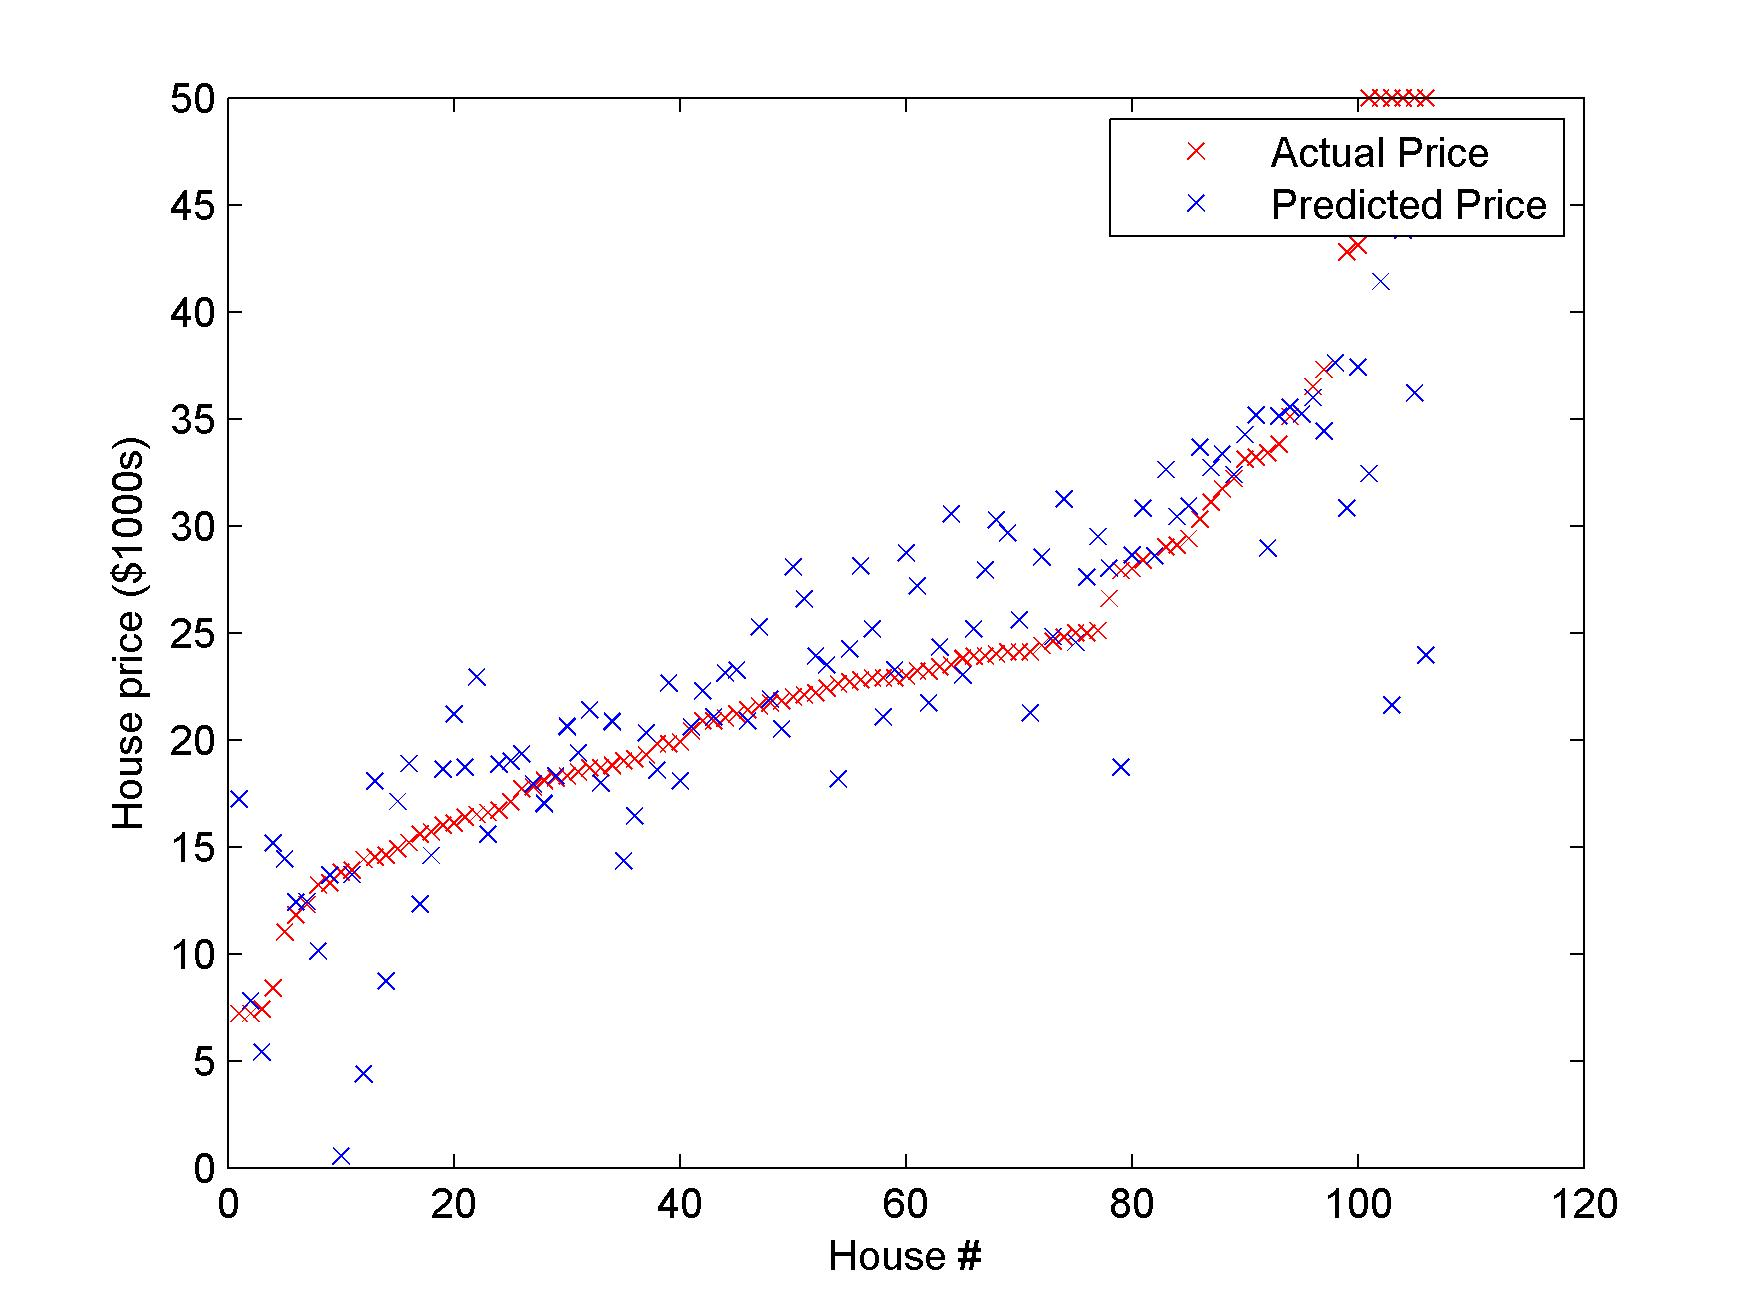
\includegraphics[scale=0.2]{./imgs/1.jpg}
\noindent
The $\mathit{linear}$\underline{  }$\mathit{regression.m}$ file is: \\
\noindent
\DefineShortVerb[fontfamily=courier,fontseries=m]{\$} 
\DefineShortVerb[fontfamily=courier,fontseries=b]{\#}               
\hspace*{-1.6em}{\scriptsize 1}$  $\color{mblue}$function$\color{black}$ [f,g] = linear_regression(theta, X,y)$\\
\hspace*{-1.6em}{\scriptsize 2}$    $\color{mgreen}$%$\color{black}$$\\
\hspace*{-1.6em}{\scriptsize 3}$    $\color{mgreen}$% Arguments:$\color{black}$$\\
\hspace*{-1.6em}{\scriptsize 4}$    $\color{mgreen}$%   theta - A vector containing the parameter values to optimize.$\color{black}$$\\
\hspace*{-1.6em}{\scriptsize 5}$    $\color{mgreen}$%   X - The examples stored in a matrix.$\color{black}$$\\
\hspace*{-1.6em}{\scriptsize 6}$    $\color{mgreen}$%       X(i,j) is the i'th coordinate of the j'th example.$\color{black}$$\\
\hspace*{-1.6em}{\scriptsize 7}$    $\color{mgreen}$%   y - The target value for each example.  y(j) is the target for example j.$\color{black}$$\\
\hspace*{-1.6em}{\scriptsize 8}$    $\color{mgreen}$%$\color{black}$$\\
\hspace*{-1.6em}{\scriptsize 9}$    $\\
\hspace*{-2em}{\scriptsize 10}$    m=size(X,2);$\\
\hspace*{-2em}{\scriptsize 11}$    n=size(X,1);$\\
\hspace*{-2em}{\scriptsize 12}$  $\\
\hspace*{-2em}{\scriptsize 13}$    f=0;$\\
\hspace*{-2em}{\scriptsize 14}$    g=zeros(size(theta));$\\
\hspace*{-2em}{\scriptsize 15}$    $\color{mgreen}$% f: cost function sum , g:gradient sum$\color{black}$$\\
\hspace*{-2em}{\scriptsize 16}$   $\color{mblue}$for$\color{black}$ row = 1:m$\\
\hspace*{-2em}{\scriptsize 17}$        curr_x = X(:,row);$\\
\hspace*{-2em}{\scriptsize 18}$        curr_y = y(:,row);$\\
\hspace*{-2em}{\scriptsize 19}$        f = f + (1/2).*(theta'*curr_x-curr_y)^2;$\\
\hspace*{-2em}{\scriptsize 20}$        g = g + curr_x.*(theta'*curr_x-curr_y);$\\
\hspace*{-2em}{\scriptsize 21}$   $\color{mblue}$end$\color{black}$$\\
\hspace*{-2em}{\scriptsize 22}$  $\color{mgreen}$% another version:vectorization$\color{black}$$\\
\hspace*{-2em}{\scriptsize 23}$  $\color{mgreen}$%   h = theta' * X - y;$\color{black}$$\\
\hspace*{-2em}{\scriptsize 24}$  $\color{mgreen}$%   f = (1/2) * h * h';$\color{black}$$\\
\hspace*{-2em}{\scriptsize 25}$  $\color{mgreen}$%   g = X*h';$\color{black}$$\\ 

\UndefineShortVerb{\$} 
\UndefineShortVerb{\#}


\section{Logistic Regression}
In this section,We will use logistic regression to solve a classification problem. In linear regression, we tried to predict the value of $\bm{y}^{(i)}$ for the $\mathit{i}$'th example $\bm{x}^{(i)}$ using a linear function $\bm{y}=\bm{h}_{\bm{\theta}}(\bm{x}) = \bm{\theta}^T\bm{x}$. This is a continuous-valued problem.
For 2-class problems,we use logistic regression which outputs denote the probability for each class as the form:\\
$$\bm{P}(\bm{y} = 1|\bm{x}) = \bm{h}_{\bm{\theta}}(\bm{x}) = 
\dfrac{1}{1+\mathbf{exp}(-\bm{\theta}^T\bm{x})} = \sigma(\bm{\theta}^T\bm{x})$$
$$\bm{P}(\bm{y} = 0|\bm{x}) = 1-\bm{h}_{\bm{\theta}}(\bm{x})$$\\
We use cross entropy to design the cost function:
$$\bm{J}(\bm{\theta}) = -\sum_{i}(\bm{y}^{(i)}log(\bm{h}_{\bm{\theta}}(\bm{x}^{(i)})) + 
(1 - \bm{y}^{(i)})log(1 - \bm{h}_{\bm{\theta}}(\bm{x}^{(i)})))$$
\noindent
The gradient of $\bm{J}(\bm{\theta})$ and written in its vector form is:
$$\nabla_{\bm{\theta}}\bm{J}(\bm{\theta}) = \sum_{i}\bm{x}^{(i)}(\bm{h}(\bm{x}^{(i)}) - \bm{y}^{(i)})$$\\
This is essentially the same as the gradient for linear regression except that the hypothesis function.
\subsection{Matlab Implementation}
There will involve 5 files:\\
1. $\mathit{ex1b}$\underline{  }$\mathit{logreg.m}$:  the main file, to optimize the cost function, train and test the model.\\
2. $\mathit{loadMNISTImages.m}$ $\mathit{ex1}$\underline{  }$\mathit{load}$\underline{  }$\mathit{minst.m}$: $\mathit{ex1}$\underline{  }$\mathit{load}$\underline{  }$\mathit{minst.m}$ call $\mathit{loadMNISTImages.m}$ function to load MNIST data, return train and test data set. Data form description: train data, a structure, containing 2 constants, X with 784*12665 and y with 1*12665, in which 12665 is train sample numbers. Test data set have the same form with 2115 train samples.\\
3. $\mathit{logistic}$\underline{  }$\mathit{regression.m}$: computing the cost function and its gradient. initializing the $\bm{\theta}$ is a 785*1 random vector, after transpose, multiplied with X to get results passed to $\mathit{sigmoid}$ function. Finally we get the computed feedforward function in which each element denote a probability correspondingly for a sample belongs to a certain class. Compared to the true results, we want to compute the cost function in order to get the gradient. \\
NOTE: the shape of gradient matrix $\bm{\theta}$(in codes is $\bm{g}$) is just the same as $\bm{x}$.$\mathit{f}$ is just a variable. \\

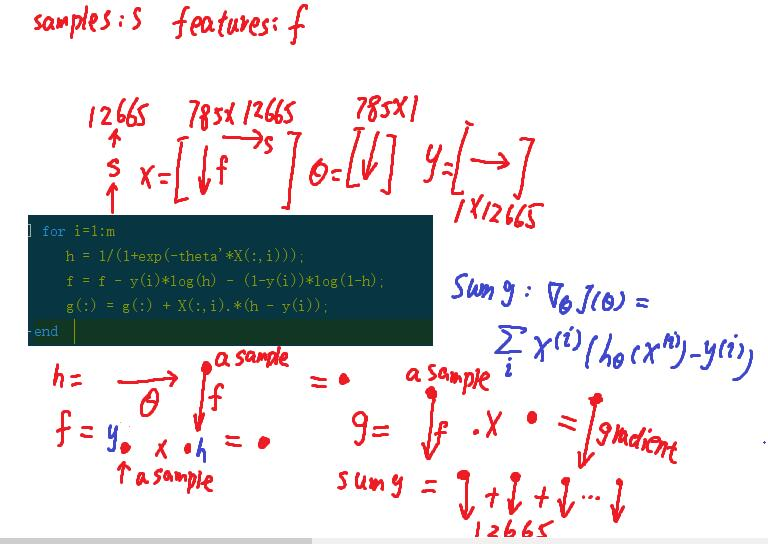
\includegraphics[scale = 0.7]{./imgs/2.jpg}\\
\\
\noindent
Vectorized version is:\\
\DefineShortVerb[fontfamily=courier,fontseries=m]{\$} 
\DefineShortVerb[fontfamily=courier,fontseries=b]{\#} 
\noindent     
\hspace*{-2em}{\scriptsize 1}$	h = 1./(1+exp(-theta' * X));$\\
\hspace*{-2em}{\scriptsize 2}$	f = -y * log(h)'-(1-y)*(log(1-h)')$\\
\hspace*{-2em}{\scriptsize 3}$	g = X * (h - y)'$\\

\UndefineShortVerb{\$}
\UndefineShortVerb{\#}
\includegraphics[scale = 0.6]{./imgs/3.pdf}\\
\noindent
4. $\mathit{binary\_classifiler\_accuracy.m}$: to calculate the model classification accuracy. Multiplied $\bm{X}$ input by the optimized $\bm{\theta}$ to get the output. If output is bigger than 0.5, that is to say classification correct.\\
\section{Debugging: Gradient Checking}
Sometimes, we need to check the gradient of objective function manually to insure that our optimization algorithm works correctly. Basically, according to derivative definition, for a extremely small $\epsilon$, we have:
$$\bm{g(\theta)} \approx \frac{\bm{J}(\bm{\theta}+\epsilon) - \bm{J}(\bm{\theta}-\epsilon)}{2 \times \epsilon}$$\\
Because $\bm{\theta}$ is a vector, if we want to check the $\mathit{i}$-th element of $\bm{g}$ vector, just:\\
$$\bm{g}_\mathit{i}(\bm{\theta}) \approx \frac{\bm{J}(\bm{\theta}^{\mathit{i+}}) - \bm{J}(\bm{\theta}^{\mathit{i-}})}{2 \times \epsilon}$$\\
Where
$$\bm{\theta^{\mathit{i\pm}}} = \bm{\theta} \pm \epsilon \times \bm{\vec{e}}_i $$
in which, $\vec{e}_i$ is the $\mathit{i}$-th basis vector of the same dimension as $\bm{\theta}$, with a "1" in the $\mathit{i}$-th position and "0"s everywhere else.

\subsection{Matlab Implementation}
We create a file called $\mathit{grad\_check.m}$. In anywhere, We just pass the optimized function, initialized $\theta$, number checks, and train data set to the $\mathit{grad\_check.m}$ function. The number checks mean that how many times we want to check the gradient of random selected dimension of $\theta$. Using form likes:

\DefineShortVerb[fontfamily=courier,fontseries=m]{\$} 
\DefineShortVerb[fontfamily=courier,fontseries=b]{\#} 
\noindent
\hspace*{-2em}{\scriptsize 1}$  error = grad_check(@logistic_regression_vec,$\color{mblue}$ ...$\color{black}$$\\
\hspace*{-2em}{\scriptsize 2}$      theta, 10, train.X, train.y)$\\

\noindent                       
\hspace*{-1.6em}{\scriptsize 1}$  $\color{mblue}$function$\color{black}$ average_error = grad_check(fun, theta0, num_checks, varargin)$\\
\hspace*{-1.6em}{\scriptsize 2}$    delta=1e-3; $\\
\hspace*{-1.6em}{\scriptsize 3}$    sum_error=0;$\\
\hspace*{-1.6em}{\scriptsize 4}$    fprintf($\color{mred}$' Iter       i             err'$\color{black}$);$\\
\hspace*{-1.6em}{\scriptsize 5}$    fprintf($\color{mred}$'           g               g_estimated               f\n'$\color{black}$)$\\
\hspace*{-1.6em}{\scriptsize 6}$    $\color{mblue}$for$\color{black}$ i=1:num_checks$\\
\hspace*{-1.6em}{\scriptsize 7}$      T = theta0;$\\
\hspace*{-1.6em}{\scriptsize 8}$      j = randsample(numel(T),1);$\\
\hspace*{-1.6em}{\scriptsize 9}$      T0=T; $\color{mred}$T0(j) = T0(j)-delta;$\color{black}$$\\
\hspace*{-2em}{\scriptsize 10}$      T1=T; $\color{mred}$T1(j) = T1(j)+delta;$\color{black}$$\\
\hspace*{-2em}{\scriptsize 11}$      $\\
\hspace*{-2em}{\scriptsize 12}$      [f,g] = fun(T, varargin{:});$\\
\hspace*{-2em}{\scriptsize 13}$      f0 = fun(T0, varargin{:});$\\
\hspace*{-2em}{\scriptsize 14}$      f1 = fun(T1, varargin{:});$\\
\hspace*{-2em}{\scriptsize 15}$      g_estimated = (f1-f0) / (2*delta);$\\
\hspace*{-2em}{\scriptsize 16}$      error = abs(g(j) - g_estimated);$\\
\hspace*{-2em}{\scriptsize 17}$      fprintf($\color{mred}$'% 5d  % 6d % 15g % 15f % 15f % 15f\n'$\color{black}$,$\color{mblue}$ ...$\color{black}$$\\
\hspace*{-2em}{\scriptsize 18}$              i,j,error,g(j),g_estimated,f);$\\
\hspace*{-2em}{\scriptsize 19}$      sum_error = sum_error + error;$\\
\hspace*{-2em}{\scriptsize 20}$    $\color{mblue}$end$\color{black}$$\\
\hspace*{-2em}{\scriptsize 21}$    average_error = sum_error/num_checks;$\\ 

\UndefineShortVerb{\$} 
\UndefineShortVerb{\#}
\section{Softmax Regression}
We use logistic regression classifier to distinguish between two kinds of hand-written digits. For multiple classes, we use softmax regression classifier. For $\bm{y}^{(i)} \in \mathfrak{R}^K$ (K classes), normalized the hypothesis distribution:
$$\bm{h_{\theta}(x)} = \frac{1}{\sum_{j=1}^{K}\mathbf{exp}(\bm{\theta}^{(j)T}\bm{x})} \left[\begin{matrix}
\mathbf{exp}(\bm{\theta}^{(1)T}\bm{x}) \\
\mathbf{exp}(\bm{\theta}^{(2)T}\bm{x}) \\
\vdots \\
\mathbf{exp}(\bm{\theta}^{(K)T}\bm{x})
\end{matrix}\right]$$
\noindent
Note that the $\bm{\theta}$ is a $\mathit{n}$-by-$\mathit{K}$ matrix, $\mathit{n}$ denoted the input feature dimensions of $\bm{x}$. Where $\bm{\theta} = [\bm{\theta^{(1)}} \bm{\theta^{(2)}} ... \bm{\theta^{(K)}} ]$\\
\subsection{Cost Function and Its properties}
From my point of view, softmax regression is a two layers neural networks, and the $\bm{\theta}$ can be seen as the weigh of the networks. In the equation below, $\bm{1\{\bullet\}}$ is the indicator function \textbf{1\{a true statement\} = 1}, and \textbf{1\{a false statement\} = 0}. That is to say when $\bullet$ is true, the $\bm{1\{\bullet\}}$ outputs 1. Our cost function will be:
$$\bm{J(\theta)} = -\bigg[\sum_{i = 1}^{m}\sum_{k=1}^{K}1\{\bm{y}^{(i) = k}\}log\frac{\mathbf{exp}(\bm{\theta}^{(k)T}\bm{x}^{(i)})}{\sum_{j=1}^{K}\mathbf{exp}(\bm{\theta}^{(k)T}\bm{x}^{(i)})}\bigg]$$
When K = 2, the cost function of softmax regression becomes:
$$\bm{J}(\bm{\theta}) = -\sum_{i}(\bm{y}^{(i)}log(\bm{h}_{\bm{\theta}}(\bm{x}^{(i)})) + 
(1 - \bm{y}^{(i)})log(1 - \bm{h}_{\bm{\theta}}(\bm{x}^{(i)})))$$
Which is the logistic regression cost function.
The gradient of softmax regression cost function is a Hessian matrix:
$$\nabla_{{\bm{\theta}}^{(k)}}\bm{J}(\bm{\theta}) = - \sum_{i=1}^{m}\bigg[\bm{x}^{(i)}\bigg(1\{\bm{y}^{(i)} = k\} - \frac{\mathbf{exp}(\bm{\theta}^{(k)T}\bm{x}^{(i)})}{\sum_{j=1}^{K}\mathbf{exp}(\bm{\theta}^{(j)T}\bm{x}^{(i)})}\bigg)\bigg]$$\\
in which, $\mathit{m}$ is sample size, $\nabla_{{\bm{\theta}}^{(k)}}\bm{J}(\bm{\theta})$ is itself a vector. Softmax regression has an unusual property that is it has a "redundant" set of parameters. In other words, suppose we take each of our parameter vectors $\bm{\theta}^{(j)}$, and subtract some fixed vector $\bm{\psi}$ from it, so that every $\bm{\theta}^{(j)}$ is now replaced with $\bm{\theta}^{(j)} - \bm{\psi}$ (for every $\mathit{j} = 1,2,...,k$ ), which means $\bm{\theta}^{(j)}$ has redundant information. Let's see how it happens. For our hypothesis function $\bm{h_{\theta}(x)}$, each element in it has the form:\\
$$\frac{\mathbf{exp}(\bm{\theta}^{(k)T}\bm{x}^{(i)})}{\sum_{j=1}^{K}\mathbf{exp}(\bm{\theta}^{(j)T}\bm{x}^{(i)})}$$\\
If we subtract a $\bm{\psi}$ from $\bm{\theta}^{(k)}$ in numerator and denominator at the same time, it, saying $exp((\bm{\theta}^{(k) - \bm{\psi}})^\mathsf{T})$. Because $\mathbf{exp}$ function properties, the calculated hypothesis result is just the same as not been subtracted. In a extreme situation, suppose $\bm{\theta}^{(K)} = \bm{\psi}$, one can reduce $K \times n $ parameters to $(K-1) \times n$ parameters needed to be optimized without harming the representational power of our hypothesis.
When $K = 2$, the softmax regression becomes logistic regression. 
$$\bm{h_{\theta}(x)} = \frac{1}{\mathbf{exp}(\bm{\theta}^{(1)\mathsf{T}}\bm{x}) + \mathbf{exp}(\bm{\theta}^{(2)\mathsf{T}}\bm{x})} \left[\begin{matrix}
	\mathbf{exp}(\bm{\theta}^{(1)\mathsf{T}}\bm{x}) \\
	\mathbf{exp}(\bm{\theta}^{(2)\mathsf{T}}\bm{x}) \\
\end{matrix}\right]$$
Tasking advantage of the properties that softmax regression hypothesis is overparameterized and setting $\bm{\psi = \theta^{(2)}}$, we can subtract $\bm{\theta^{(2)}}$ from each of the two parameters, giving us
\begin{align*}
\bm{h_{\theta}(x)} &= \frac{1}{\mathbf{exp}((\bm{\theta}^{(1)} - \bm{\theta}^{(2)})^{\mathsf{T}}\bm{x}) + 1} \left[\begin{matrix}
\mathbf{exp}((\bm{\theta}^{(1)} - \bm{\theta}^{(2)})^{\mathsf{T}}\bm{x}) \\
1\\
\end{matrix}\right]\\
&= \left[\begin{matrix}
1 - \frac{1}{\mathbf{exp}((\bm{\theta}^{(1)} - \bm{\theta}^{(2)})^{\mathsf{T}}\bm{x}) + 1} \\
\frac{1}{\mathbf{exp}((\bm{\theta}^{(1)} - \bm{\theta}^{(2)})^{\mathsf{T}}\bm{x}) + 1}\\
\end{matrix}\right]\\
&= \left[\begin{matrix}
1 - \frac{1}{\mathbf{exp}(\bm{-\theta}^{'\mathsf{T}}\bm{x}) + 1} \\
\frac{1}{\mathbf{exp}(\bm{-\theta}^{'\mathsf{T}}\bm{x}) + 1}\\
\end{matrix}\right]\quad (\textrm{if we denote}\:\bm{\theta}^{(2)} - \bm{\theta}^{(1)} = \bm{-\theta}^{'})
\end{align*}
From the above derivation, we find that softmax regression predicts the probability of one of the classes as $\frac{1}{\mathbf{exp}(\bm{-\theta}^{'\mathsf{T}}\bm{x}) + 1}$, and that of the other class as $1 - \frac{1}{\mathbf{exp}(\bm{-\theta}^{'\mathsf{T}}\bm{x}) + 1}$, same as logistic regression.
\subsection{Matlab Implementation}
It will involve three files:\\
1. $\mathit{ex1c\_softmax.m}$: the main file.\\
2. $\mathit{multi\_classifier\_accuracy.m}$: to estimate the model.
3. $\mathit{softmax\_regression\_vec.m}$: to compute the cost fucntion and its gradients. The unvectorized core codes are:\\
\DefineShortVerb[fontfamily=courier,fontseries=m]{\$} 
\DefineShortVerb[fontfamily=courier,fontseries=b]{\#} 
\noindent
\hspace*{-2em}{\scriptsize 1}$   $\color{mblue}$for$\color{black}$ i=1:m$\\     
\hspace*{-2em}{\scriptsize 2}$	label = y(i);$\\
\hspace*{-2em}{\scriptsize 3}$	p_k_1 = exp(theta'*X(:,i));$\\
\hspace*{-2em}{\scriptsize 4}$	p_norm = p_k_1 ./ sum(p_k_1);$\\
\hspace*{-2em}{\scriptsize 5}$	f = f - log(p_norm(label));$\\
\hspace*{-2em}{\scriptsize 6}$       $\color{mblue}$for$\color{black}$ j=1:num_classes$\\  
\hspace*{-2em}{\scriptsize 7}$            g(:,j) = g(:,j) + X(:,i).*(p_norm(j));$\\
\hspace*{-2em}{\scriptsize 8}$       $\color{mblue}$end$\color{black}$$\\
\hspace*{-2em}{\scriptsize 9}$	g(:,label) = g(:,label) - X(:,i);$\\
\hspace*{-2em}{\scriptsize 10}$   $\color{mblue}$end$\color{black}$$\\
\hspace*{-2em}{\scriptsize 11}$  f = f./m;$\\
\hspace*{-2em}{\scriptsize 12}$  g(:,num_classes) = [];$\\
\hspace*{-2em}{\scriptsize 13}$  g=g./m;$\\
\hspace*{-2em}{\scriptsize 14}$  $\color{mgreen}$% make gradient a vector for minFunc$\color{black}$$\\
\hspace*{-2em}{\scriptsize 15}$  g=g(:);$\\
\UndefineShortVerb{\$}
\UndefineShortVerb{\#}
\noindent
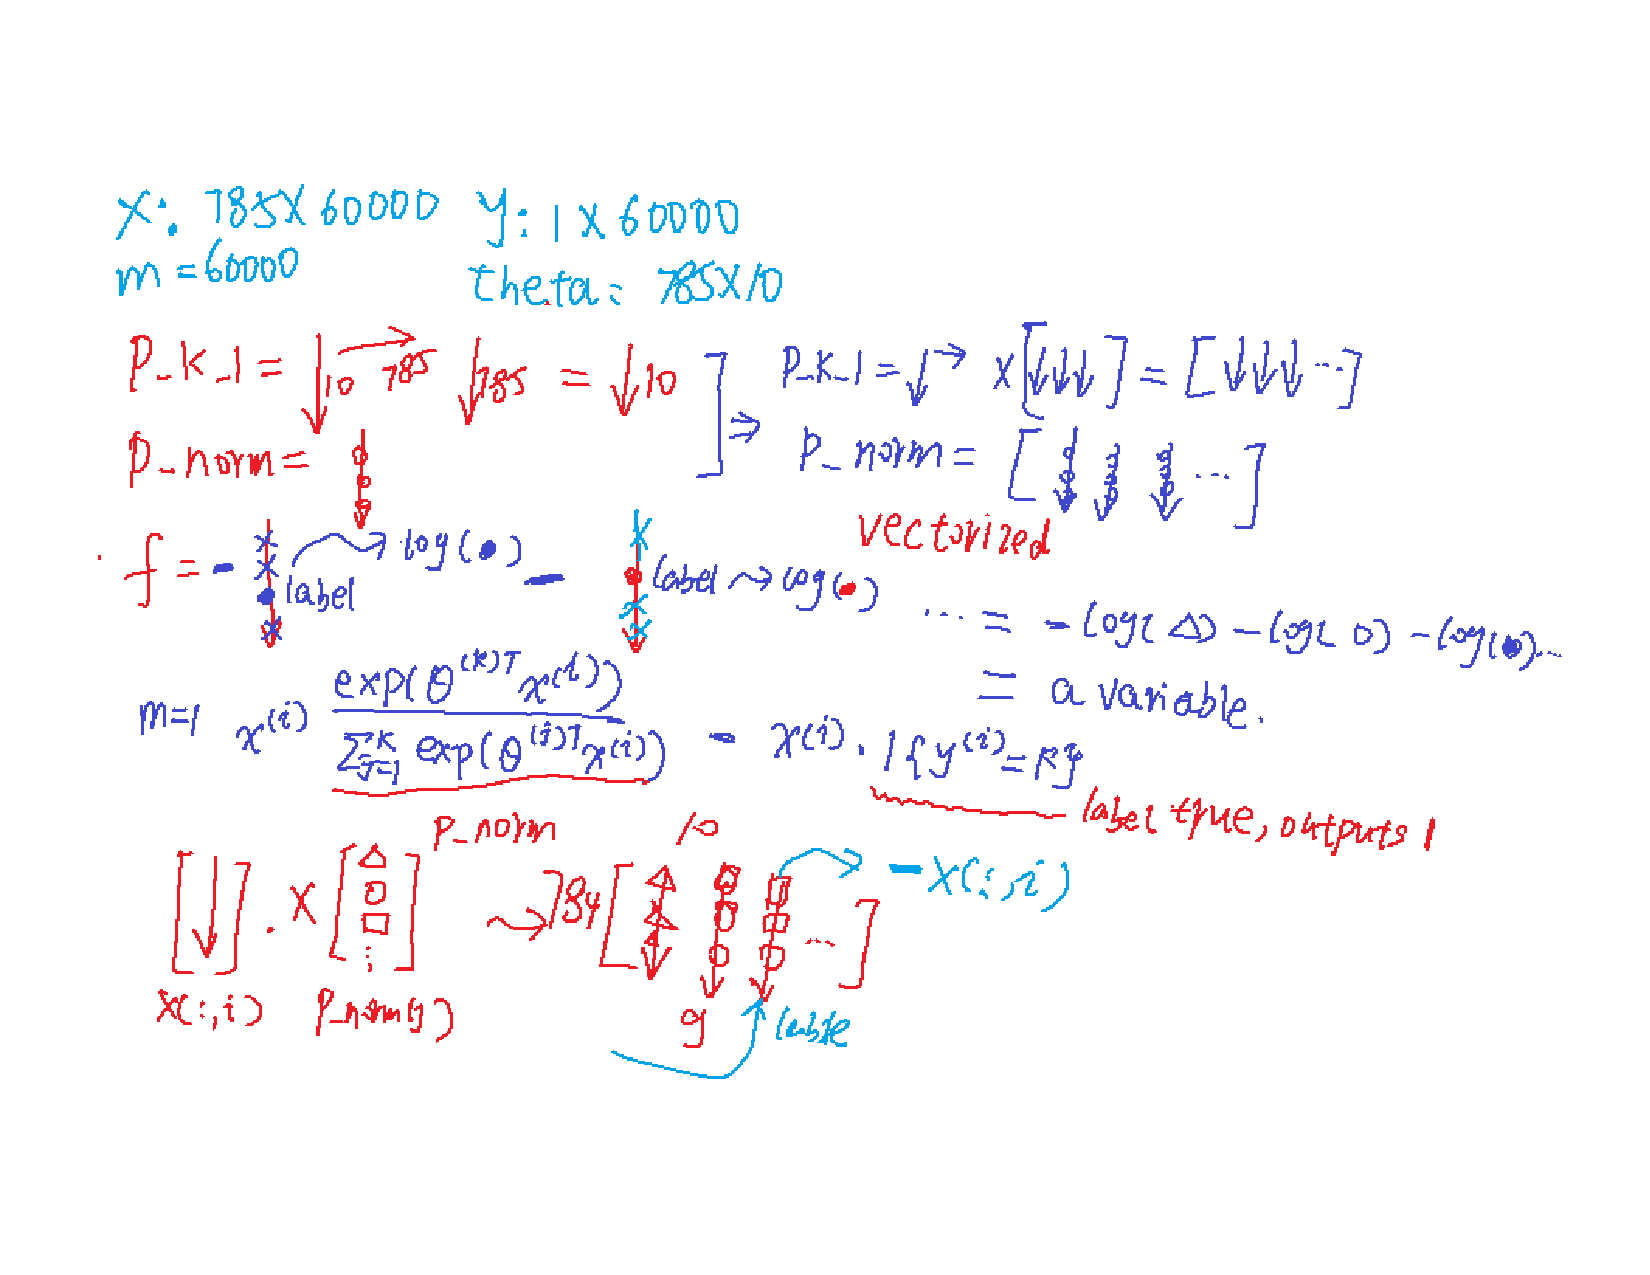
\includegraphics[scale = 0.6]{./imgs/4.pdf}
Note: we would handle all 10 digit classes instead 2 classes as in the previous section. According to softmax regression properties, the last class corresponding to its gradient could be set 0, meaning the 10th class is left out of $\bm{\theta}$.

\section{Neural Network and Backpropagation Algorithm}
In this section, we will learn a model called Neural Network(NN), and see how does such model can help us to compute graph-based model. We will from another point of view to see softmax regression. First, I would introduce basic mathematical notations, and then briefly describe the network architecture.
\begin{itemize}
\item[1.] $\bm{W}_{i,j}^{(l)}$: the parameter(or weigh) associated with the connection between unit $j$ in layer $l$, and unit $i$ in layer $l+1$. The network connection direction is from $j$ to $i$.
\item[2.] $\bm{b}_{i}^{(l)}$: the bias associated with unit $i$ in layer $l+1$.
\item[3.] $\bm{a}_{i}^{l}$: activation of unit $i$ in layer $l$. Especially, $\bm{a}_{i}^{(1)} = \bm{x}_i$.
\item[4.] $\bm{W,b}$: combination of all the $\bm{W}_{i,j}^{(l)}$ and $\bm{b}_{i}^{(l)}$, are total parameters of network we basically want to learn.
\item[5.] $m$: training example size.
\item[6.] $\lambda$: weigh decay parameter.
\item[7.] $\bm{\delta_i^{(l)}}$: error term, the core of our backpropagation algorithm, which measures how much that node($i$-th node in layer $l$) responsible for any errors in our output.
\end{itemize}
The cost function(one-half squared-error cost function, with $\bm{L2}$ regularization) for the network to be:
\begin{align*}
\bm{J}(\bm{W,b}) &= \bigg[\frac{1}{m}\sum_{i=1}^{m}\bm{J}(\bm{W,b};\bm{x}^{(i)},\bm{y}^{(i)})\bigg] + \frac{\lambda}{2}\sum_{l=1}^{n_{l-1}}\sum_{i=1}^{s_l}\sum_{j=1}^{s_{l+1}}\Big(\bm{W}_{ji}^{(l)}\Big)^2\\
&= \bigg[\frac{1}{m}\sum_{i=1}^{m}\Big(\frac{1}{2}\parallel\bm{h_{W,b}}(\bm{x}^{(i)}) - \bm{y}^{(i)}\parallel^2\Big)\bigg] + \frac{\lambda}{2}\sum_{l=1}^{n_{l-1}}\sum_{i=1}^{s_l}\sum_{j=1}^{s_{l+1}}\Big(\bm{W}_{ji}^{(l)}\Big)^2
\end{align*}
As $\bm{\delta_i^{(l)}}$ is a very important term in our backpropagation algorithm, we now formally describe how to compute it:
\begin{itemize}
\item[1.] Perform a feedforward pass, computing The activations for layers $\bm{L_2}$, $\bm{L_3}$, and so on up to output layer $\bm{L_{n_{l}}}$.
\item[2.]  For each output unit $i$ in layer $n_l$ (the output layer), set\\
$$\bm{\delta}_i^{(n_l)} = \frac{\partial}{\partial \bm{z}_i^{(n_l)}}\frac{1}{2}\parallel\bm{y} - \bm{h_{W,b}}(\bm{x})\parallel^2 = -(\bm{y_i} - \bm{a}_i^{(n_l)}) \centerdot \bm{f'}(\bm{z}_i^{(n_l)})$$
in which, $\bm{z}^{l+1} = \bm{W}^{(l)}a^{(l)} + b^{(l)}$, $\bm{a}^{(l+1)}  = \bm{f}(\bm{z}^{(l+1)})$.
\item[3.] For $l = n_l-1, n_l-2, n_l-3,...,2$
	For each node $i$ in layer $l$, set
	$$\bm{\delta}_i^{(l)} = \Big(\sum_{j=1}^{s_{l+1}}\bm{W}_{ji}^{(l)}\bm{\delta}_j^{(l+1)}\Big)\bm{f'}(\bm{z}_i^{(l)})$$
\item[4.] Compute the desired partial derivatives, which are given as:
$$\frac{\partial}{\partial\bm{W}_{ij}^{(l)}}\bm{J(W,b;x,y)} = \bm{a}_j^{(l)}\delta_{i}^{(l+1)}$$
$$\frac{\partial}{\partial\bm{b}_{i}^{(l)}}\bm{J(W,b;x,y)} = \delta_{i}^{(l+1)}$$
\end{itemize}
Finally, we can re-write the algorithm using matrix-vectorial notation. We will use "$\bullet$" to denote the element-wise product operator. We also do The same for $\bm{f'(\bullet)}$(so that $\bm{f'([z_1,z_2]) = [f'(z_1),f'(z_2)]}$).
For step2, after vetorizing, we get (just eliminate $i$ notation)
$$\bm{\delta}^{(n_l)} = -(\bm{y} - \bm{a}^{(n_l)}) \bullet \bm{f'}(\bm{z}^{(n_l)})$$
For step3, the equation can be re-write as:
$$\bm{\delta}^{(l)} = \Big((\bm{W}^{(l)})^T\bm{\delta}^{(l+1)}\Big)\bullet\bm{f'}(\bm{z}^{(l)})$$
For step4,
$$\nabla_{\bm{W}^{(l)}}\bm{J(W,b;x,y)} = \delta^{(l+1)}(\bm{a}^{(l)})^T$$
$$\nabla_{\bm{b}^{(l)}}\bm{J(W,b;x,y)} = \delta^{(l+1)}$$
If we use sigmoid activation, $\bm{f'(z_i^{(l)})} = \bm{a_i^{(l)}(1 - a_i^{(l)})}$.\\
\subsection{BackPropogation Implementation Using Matlab }
%\includegraphics[scale = 0.6]{3.pdf}
Based on the previous section, we will train a neural network classifier to classify the 10 digits in the MNIST dataset. First, let's define a neural network We will work for it later. We have a network with a layer of 784 input units, a layer of 10 output units and a single hidden layer of 256 hidden units.
\begin{itemize}
\item {\color{blue}\emph{\texttt{run\textunderscore train.m}}}\\
The main script, to load MNIST data set, setup random initial weighs, make cost function optimized and compute accuracy on the test and train set.
\item {\color{blue}\emph{\texttt{initialize\textunderscore weights.m}}}\\
Initialling the weights between each layer, the results are stored in "stack" variable. As the network has 3 layers, neurons of each layer are 784-256-1. The "stack" variable has such a form: stack<1$\times$2 cell>, stack(1, 1) has variables of $\bm{W}$<256$\times$784 double> and $\bm{b}$<256$\times$1 double>, stack(1, 2) has variables of $\bm{W}$<10$\times$256 double> and $\bm{b}$<10$\times$1 double>.
\item {\color{blue}\emph{\texttt{params2stack.m}}} {\color{blue}\emph{\texttt{stack2params.m}}}
Converts a flattened parameter vector into a nice "stack" structure or flattens a stack to a vector for us to work with. For example, if we use "stack = params2stack(params, ei)", the "params" is our object we want to convert, and the "ei" is an auxiliary variable(maybe a cell structure in matlab) which tells us the configuration of the network we need to satisfy after converted. The total size of "params" here is 203430, according to "ai" structure, we have $203430=256\times784+256+10\times256+10$. Because "minFunc" only can deal with parameters vector, we need such mechanism to convert back and forth.
\item {\color{blue}\emph{\texttt{supervised\textunderscore dnn\textunderscore cost.m}}}\\
Our core function, to slave cost and gradient computation. It contains three main components, forward prop, cost computation and gradients computed using backpropagation.\\
\DefineShortVerb[fontfamily=courier,fontseries=m]{\$} 
\DefineShortVerb[fontfamily=courier,fontseries=b]{\#} 

\noindent                                                                                                                                        
\hspace*{-1.6em}{\scriptsize 1}$  $\color{mblue}$function$\color{black}$ [ cost, grad, pred_prob] = supervised_dnn_cost( theta, ei,...$\\
\hspace*{-1.6em}{\scriptsize 2}$      data, $\color{mred}$labels, pred_only)$\color{black}$$\\
\hspace*{-1.6em}{\scriptsize 3}$  $\color{mgreen}$%SPNETCOSTSLAVE Slave cost function for simple phone net$\color{black}$$\\
\hspace*{-1.6em}{\scriptsize 4}$  $\color{mgreen}$%   Does all the work of cost / gradient computation$\color{black}$$\\
\hspace*{-1.6em}{\scriptsize 5}$  $\color{mgreen}$%   Returns cost broken into cross-entropy, weight norm, and prox reg$\color{black}$$\\
\hspace*{-1.6em}{\scriptsize 6}$  $\color{mgreen}$%        components (ceCost, wCost, pCost)$\color{black}$$\\
\hspace*{-1.6em}{\scriptsize 7}$  $\\
\hspace*{-1.6em}{\scriptsize 8}$  $\color{mgreen}#%% default values#\color{black}$$\\
\hspace*{-1.6em}{\scriptsize 9}$  po = false;$\\
\hspace*{-2em}{\scriptsize 10}$  $\color{mblue}$if$\color{black}$ exist($\color{mred}$'pred_only'$\color{black}$,$\color{mred}$'var'$\color{black}$)$\\
\hspace*{-2em}{\scriptsize 11}$    po = pred_only;$\\
\hspace*{-2em}{\scriptsize 12}$  end;$\\
\hspace*{-2em}{\scriptsize 13}$  $\\
\hspace*{-2em}{\scriptsize 14}$  $\color{mgreen}#%% reshape into network#\color{black}$$\\
\hspace*{-2em}{\scriptsize 15}$  stack = params2stack(theta, ei);$\\
\hspace*{-2em}{\scriptsize 16}$  numHidden = numel(ei.layer_sizes) - 1;$\\
\hspace*{-2em}{\scriptsize 17}$  hAct = cell(numHidden+1, 1);$\color{mgreen}$%hAct is <2*1 cell>$\color{black}$$\\
\hspace*{-2em}{\scriptsize 18}$  gradStack = cell(numHidden+1, 1);$\color{mgreen}$%gradStack is <2*1 cell>$\color{black}$$\\
\hspace*{-2em}{\scriptsize 19}$  $\color{mgreen}#%% forward prop#\color{black}$$\\
\hspace*{-2em}{\scriptsize 20}$  $\color{mgreen}#%%% YOUR CODE HERE %%%#\color{black}$$\\
\hspace*{-2em}{\scriptsize 21}$  m = size(data,2);$\color{mgreen}$%m=60000$\color{black}$$\\
\hspace*{-2em}{\scriptsize 22}$  m_inv = 1/m;$\\
\hspace*{-2em}{\scriptsize 23}$  $\color{mblue}$for$\color{black}$ l = 1:(numHidden+1)$\\
\hspace*{-2em}{\scriptsize 24}$      $\color{mblue}$if$\color{black}$ l==1$\\
\hspace*{-2em}{\scriptsize 25}$          hAct{l} = data; $\color{mgreen}$% just store input data<784*60000>$\color{black}$$\\
\hspace*{-2em}{\scriptsize 26}$      $\color{mblue}$else$\color{black}$$\\
\hspace*{-2em}{\scriptsize 27}$  $\color{mgreen}$% when run to here, l=2.$\color{black}$$\\
\hspace*{-2em}{\scriptsize 28}$  $\color{mgreen}$% stack{l-1}.W <256*784>,hAct{l-1}=hAct{1} <784*60000>$\color{black}$$\\
\hspace*{-2em}{\scriptsize 29}$  $\color{mgreen}$% after multiplying,<256*60000>meaning demension from $\color{black}$$\\
\hspace*{-2em}{\scriptsize 30}$  $\color{mgreen}$% 784 reduce to 256. stack{l-1}.b=stack{1} <256*1>$\color{black}$$\\
\hspace*{-2em}{\scriptsize 31}$  $\color{mgreen}$% repmat(stack{l-1}.b,[1,m]) is <256*60000>,meaning row direction$\color{black}$$\\
\hspace*{-2em}{\scriptsize 32}$  $\color{mgreen}$% repeats 1 times and column direction repeats 60000 times.$\color{black}$$\\
\hspace*{-2em}{\scriptsize 33}$  $\color{mgreen}$% because for a sample we have 256 dimensions in hidden layer,so$\color{black}$$\\
\hspace*{-2em}{\scriptsize 34}$  $\color{mgreen}$% we have 256 neurons,meaning has 256 bias for a sample.$\color{black}$$\\
\hspace*{-2em}{\scriptsize 35}$  $\color{mgreen}$% here hAct{l} is "L",l=2, not number 1.$\color{black}$$\\
\hspace*{-2em}{\scriptsize 36}$          hAct{l} = stack{l-1}.W * hAct{l-1} +$\color{mblue}$ ...$\color{black}$$\\
\hspace*{-2em}{\scriptsize 37}$              repmat(stack{l-1}.b,[1,m]);$\\
\hspace*{-2em}{\scriptsize 38}$          $\color{mblue}$if$\color{black}$ strcmp(ei.activation_fun,$\color{mred}$'logistic'$\color{black}$)$\\
\hspace*{-2em}{\scriptsize 39}$              hAct{l} = sigmoid(hAct{l});$\\
\hspace*{-2em}{\scriptsize 40}$          $\color{mblue}$elseif$\color{black}$ strcmp(ei.activation_fun,$\color{mred}$'tanh'$\color{black}$)$\\
\hspace*{-2em}{\scriptsize 41}$              hAct{l} = tanh(hAct{l});$\\
\hspace*{-2em}{\scriptsize 42}$          $\color{mblue}$elseif$\color{black}$ strcmp(ei.activation_fun,$\color{mred}$'rlu'$\color{black}$)$\\
\hspace*{-2em}{\scriptsize 43}$              hAct{l}(hAct{l}<0) = 0;$\\
\hspace*{-2em}{\scriptsize 44}$          $\color{mblue}$end$\color{black}$$\\
\hspace*{-2em}{\scriptsize 45}$      $\color{mblue}$end$\color{black}$$\\
\hspace*{-2em}{\scriptsize 46}$  $\color{mblue}$end$\color{black}$$\\
\hspace*{-2em}{\scriptsize 47}$  $\color{mgreen}$% layer l=2,stack{l}.W <10,256>,hAct{l}< 256*60000>,$\color{black}$$\\
\hspace*{-2em}{\scriptsize 48}$  $\color{mgreen}$% stack{l}.b <10,1>$\color{black}$$\\
\hspace*{-2em}{\scriptsize 49}$  $\color{mgreen}$% repmat(stack{l}.b,[1,m])<10,60000>. From another perspective,$\color{black}$$\\
\hspace*{-2em}{\scriptsize 50}$  $\color{mgreen}$% the output layer mapping 256 demensions to 10 demensions.$\color{black}$$\\
\hspace*{-2em}{\scriptsize 51}$  $\color{mgreen}$% pred_prob <10*60000>$\color{black}$$\\
\hspace*{-2em}{\scriptsize 52}$  pred_prob = stack{l}.W * hAct{l} + repmat(stack{l}.b,[1,m]);$\\
\hspace*{-2em}{\scriptsize 53}$  $\color{mgreen}$% perform element-by-element binary operation for two array.$\color{black}$$\\
\hspace*{-2em}{\scriptsize 54}$  $\color{mgreen}$% max(pred_prob,[],1) <1*60000>, here, "max" function $\color{black}$$\\
\hspace*{-2em}{\scriptsize 55}$  $\color{mgreen}$% produces the maximum values along the first $\color{black}$$\\
\hspace*{-2em}{\scriptsize 56}$  $\color{mgreen}$% dimension of "pred_prob".$\color{black}$$\\
\hspace*{-2em}{\scriptsize 57}$  $\color{mgreen}$% normalizes the output to range[0,1] to represent probability.$\color{black}$$\\
\hspace*{-2em}{\scriptsize 58}$  $\color{mgreen}$% bsxfun works like it,suppose $\color{black}$$\\
\hspace*{-2em}{\scriptsize 59}$  $\color{mgreen}$% A = [1 4 6  B=[2 2 2],after bsxfun(@minus,A,B) = [-1 2 4$\color{black}$$\\
\hspace*{-2em}{\scriptsize 60}$  $\color{mgreen}$%     5 7 3]                                        3  5  2]$\color{black}$$\\
\hspace*{-2em}{\scriptsize 61}$  $\color{mgreen}$% after sigmoid function, each neuron output  $\color{black}$$\\
\hspace*{-2em}{\scriptsize 62}$  $\color{mgreen}$% a variable range[0,1],however$\color{black}$$\\
\hspace*{-2em}{\scriptsize 63}$  $\color{mgreen}$% for Softmax regression, we treat these outputs $\color{black}$$\\
\hspace*{-2em}{\scriptsize 64}$  $\color{mgreen}$% as weighed inputs,and put these outputs into $\color{black}$$\\
\hspace*{-2em}{\scriptsize 65}$  $\color{mgreen}$% exp power function and divided by its sum $\color{black}$$\\
\hspace*{-2em}{\scriptsize 66}$  $\color{mgreen}$% respectively for each sample$\color{black}$$\\
\noindent
The cost The cost function is nearly identical to the softmax regression cost function. Note that instead of making predictions from the input data x the softmax function takes as input the final hidden layer of the network \begin{equation}\label{key}
\bm{h_{W,b}(x)}
\end{equation}.
The loss function is thus:
\begin{equation*}
\bm{J(\theta)} = -\bigg[\sum_{i = 1}^{m}\sum_{k=1}^{K}1\{\bm{y}^{(i) = k}\}log\frac{\mathbf{exp}(\bm{\theta}^{(k)T}\bm{h_{W,b}(x^{(i)})})}{\sum_{j=1}^{K}\mathbf{exp}(\bm{\theta}^{(k)T}\bm{h_{W,b}(x^{(i)})})}\bigg]
\end{equation*} 
\noindent\\
\hspace*{-2em}{\scriptsize 67}$  pred_prob = bsxfun(@minus,pred_prob,max(pred_prob,[],1));$\\
\hspace*{-2em}{\scriptsize 68}$  pred_prob = exp(pred_prob);$\\
\hspace*{-2em}{\scriptsize 69}$  pred_prob = bsxfun(@rdivide, pred_prob, sum(pred_prob));$\\
\hspace*{-2em}{\scriptsize 70}$  $\\
\hspace*{-2em}{\scriptsize 71}$  $\color{mgreen}#%% return here if only predictions desired.#\color{black}$$\\
\hspace*{-2em}{\scriptsize 72}$  $\color{mblue}$if$\color{black}$ po$\\
\hspace*{-2em}{\scriptsize 73}$    cost = -1; ceCost = -1; wCost = -1; numCorrect = -1;$\\
\hspace*{-2em}{\scriptsize 74}$    grad = [];$\\
\hspace*{-2em}{\scriptsize 75}$    return;$\\
\hspace*{-2em}{\scriptsize 76}$  end;$\\
\hspace*{-2em}{\scriptsize 77}$  $\\
\hspace*{-2em}{\scriptsize 78}$  $\color{mgreen}#%% compute cost#\color{black}$$\\
\hspace*{-2em}{\scriptsize 79}$  $\color{mgreen}#%%% YOUR CODE HERE %%%#\color{black}$$\\
\hspace*{-2em}{\scriptsize 80}$  $\color{mgreen}$% groundTruth <10*60000>,meaning if groundTruth(j,i) not equal to 0, $\color{black}$$\\
\hspace*{-2em}{\scriptsize 81}$  $\color{mgreen}$% that j is the hand number label for input sample i$\color{black}$$\\
\hspace*{-2em}{\scriptsize 82}$  groundTruth = full(sparse(labels, 1:m, 1));$\\
\hspace*{-2em}{\scriptsize 83}$  $\color{mgreen}$% groundTruth <10*60000>,pred_prob <10*60000>,after sum, <1*60000>$\color{black}$$\\
\hspace*{-2em}{\scriptsize 84}$  cost = -mean(sum(groundTruth .* log(pred_prob)));$\\
\hspace*{-2em}{\scriptsize 85}$  $\color{mgreen}$% to add L2 regularization term.$\color{black}$$\\
\hspace*{-2em}{\scriptsize 86}$  ceCost = -(groundTruth - pred_prob);$\\
\hspace*{-2em}{\scriptsize 87}$  wCost = 0;$\\
\hspace*{-2em}{\scriptsize 88}$  $\color{mgreen}$% for all weighs in the network, just sum all weighs^2 up.Here wCost$\color{black}$$\\
\hspace*{-2em}{\scriptsize 89}$  $\color{mgreen}$% called weigh cost$\color{black}$$\\
\hspace*{-2em}{\scriptsize 90}$  $\color{mblue}$for$\color{black}$ l=1:(numHidden+1)$\\
\hspace*{-2em}{\scriptsize 91}$      wCost = wCost + sum(sum(stack{l}.W .^ 2));$\\
\hspace*{-2em}{\scriptsize 92}$  $\color{mblue}$end$\color{black}$$\\
\hspace*{-2em}{\scriptsize 93}$  wCost = 0.5 * ei.lambda * wCost;$\\
\hspace*{-2em}{\scriptsize 94}$  cost = cost + wCost;$\\
\hspace*{-2em}{\scriptsize 95}$  $\\
\hspace*{-2em}{\scriptsize 96}$  $\color{mgreen}#%% compute gradients using backpropagation#\color{black}$$\\
\hspace*{-2em}{\scriptsize 97}$  $\color{mgreen}#%%% YOUR CODE HERE %%%#\color{black}$$\\
\hspace*{-2em}{\scriptsize 98}$  delta = cell(numHidden+1,1);$\color{mgreen}$%delta<2*1 cell>$\color{black}$$\\
\hspace*{-2em}{\scriptsize 99}$  $\color{mblue}$for$\color{black}$ l=numHidden+1:-1:1 $\color{mgreen}$%from back to front, numHidden = 1$\color{black}$$\\
\hspace*{-2.4em}{\scriptsize 100}$      $\color{mgreen}$% layer l is 2,2==1+1,output layer backpro$\color{black}$$\\
\hspace*{-2.4em}{\scriptsize 101}$      if(l==numHidden+1)$\\
\hspace*{-2.4em}{\scriptsize 102}$          delta{l} = ceCost;$\\
\hspace*{-2.4em}{\scriptsize 103}$          $\color{mgreen}$%the residual between groundTruth and computed results$\color{black}$$\\
\hspace*{-2.4em}{\scriptsize 104}$          $\color{mgreen}$% delta{2}<10*60000>,hAct{2}<256*60000>,actually is hidden$\color{black}$$\\
\hspace*{-2.4em}{\scriptsize 105}$          $\color{mgreen}$% layer (layer 2) output (activation output).$\color{black}$$\\
\hspace*{-2.4em}{\scriptsize 106}$          $\color{mgreen}$% I AM CONFUSED AT HERE.$\color{black}$$\\
\hspace*{-2.4em}{\scriptsize 107}$          gradStack{l}.W = delta{l} * hAct{l}' .* m_inv;$\\
\hspace*{-2.4em}{\scriptsize 108}$          gradStack{l}.b = mean(delta{l},2);$\\
\hspace*{-2.4em}{\scriptsize 109}$      $\color{mblue}$else$\color{black}$$\\
\hspace*{-2.4em}{\scriptsize 110}$          $\color{mgreen}$% stack{2}.W'<60000*10>,delta{2}<10*60000>$\color{black}$$\\
\hspace*{-2.4em}{\scriptsize 111}$          delta{l} = stack{l+1}.W' * delta{l+1};$\\
\hspace*{-2.4em}{\scriptsize 112}$          $\color{mblue}$if$\color{black}$ strcmp(ei.activation_fun,$\color{mred}$'logistic'$\color{black}$)$\\
\hspace*{-2.4em}{\scriptsize 113}$              delta{l} = delta{l} .* hAct{l+1} .* (1-hAct{l+1});$\\
\hspace*{-2.4em}{\scriptsize 114}$          $\color{mblue}$elseif$\color{black}$ strcmp(ei.activation_fun,$\color{mred}$'tanh'$\color{black}$)$\\
\hspace*{-2.4em}{\scriptsize 115}$              delta{l} = delta{l} .* (1-hAct{l+1}.^2);$\\
\hspace*{-2.4em}{\scriptsize 116}$          $\color{mblue}$elseif$\color{black}$ strcmp(ei.activation_fun,$\color{mred}$'rlu'$\color{black}$)$\\
\hspace*{-2.4em}{\scriptsize 117}$              delta{l}(hAct{l+1}<0) = 0;$\\
\hspace*{-2.4em}{\scriptsize 118}$          $\color{mblue}$end$\color{black}$$\\
\hspace*{-2.4em}{\scriptsize 119}$          $\color{mgreen}$% I AM doubt here,why not consider the W2 matrix?$\color{black}$$\\
\hspace*{-2.4em}{\scriptsize 120}$          $\color{mgreen}$% l = 1$\color{black}$$\\
\hspace*{-2.4em}{\scriptsize 121}$          gradStack{l}.W = delta{l} * hAct{l}' .* m_inv +$\color{mblue}$ ...$\color{black}$$\\
\hspace*{-2.4em}{\scriptsize 122}$              ei.lambda .* stack{l}.W;$\\
\hspace*{-2.4em}{\scriptsize 123}$          gradStack{l}.b = mean(delta{l},2);$\\
\hspace*{-2.4em}{\scriptsize 124}$      $\color{mblue}$end$\color{black}$$\\
\hspace*{-2.4em}{\scriptsize 125}$  $\color{mblue}$end$\color{black}$$\\
\hspace*{-2.4em}{\scriptsize 126}$  $\\
\hspace*{-2.4em}{\scriptsize 127}$  $\color{mgreen}#%% compute weight penalty cost and gradient for non-bias terms#\color{black}$$\\
\hspace*{-2.4em}{\scriptsize 128}$  $\color{mgreen}#%%% YOUR CODE HERE %%%#\color{black}$$\\
\hspace*{-2.4em}{\scriptsize 129}$  $\\
\hspace*{-2.4em}{\scriptsize 130}$  $\color{mgreen}#%% reshape gradients into vector#\color{black}$$\\
\hspace*{-2.4em}{\scriptsize 131}$  [grad] = stack2params(gradStack);$\\
\hspace*{-2.4em}{\scriptsize 132}$  $\color{mblue}$end$\color{black}$$\\
\hspace*{-2.4em}{\scriptsize 133}$  $\\
\hspace*{-2.4em}{\scriptsize 134}$  $\color{mblue}$function$\color{black}$ sigm = sigmoid(x)$\\
\hspace*{-2.4em}{\scriptsize 135}$      sigm = 1./(1+exp(-x));$\\
\hspace*{-2.4em}{\scriptsize 136}$  $\color{mblue}$end$\color{black}$$\\ 

\UndefineShortVerb{\$} 
\UndefineShortVerb{\#}
\end{itemize} 
\section{Convolutional Neural Networks and pooing}
If you have already been familiar with convolutional neural network, here I will emphasize some important details of it only. Basically, suppose input volume is a \emph{width*height*depth} image, which width size is always the same with height, meaning that is a square shape. Filter is \emph{width\_filter*height\_filter*depth\_filter}, which always is the case that $width\_filter = height\_filter, depth = depth\_filter$. If we have $\mathit{K}$ filters, then we will get $K$ activation maps. For a activation map, suppose the padding size is for one border, it has output size $((width - width\_filter + 2*padding size)/stride+1) \times ((height - height\_filter + 2*padding size)/stride+1)$. In common settings, $K$ is always the powers of 2, e.g. 32, 64, 128. For an element in activation, we get it by element-wise product of volume \emph{width*height*depth} and \emph{width\_filter*height\_filter*depth\_filter}. For a next time, we move the filter volume a stride , do the element-wise product, and get another element of the activation map. If we have a $1\times1$ filter with depth of $D$, the  corresponding activation map size will not change compared to input volume but its depth to $D$.\\
Pooling, also known as downshampling, captures a feature-invariance property. Say we have a activation map $m\times m$ needed to be pool. If we implement $n\times n$ pooling, Then, our output has $(m\div n) \times (m\div n)$ regions. For a region, we take $n\times n$ mean (or maximum) feature pooling over $m\times m$ activation map to obtain the pooled convolved features.
\subsection{Implement convolution and Pooling}
There are somes implementation tips. If we use {\color{red}conv2(image, W)} MATLAB function, as MATLAB will first "flip" {\color{red}W} before convolving {\color{red}W} with {\color{red}image}, we need to rotate it twice {\color{red}rot90} before put it into {\color{red}conv2} function, e.g.:\\
\begin{equation*}
\left[\begin{matrix}
1 &2 &3 \\
4 &5 &6 \\
7 &8 &9 \\
\end{matrix}\right] \xLongleftrightarrow[flip]{rotate-twice}
\left[\begin{matrix}
9 &8 &7 \\
6 &5 &4 \\
3 &2 &1 \\
\end{matrix}\right] 
\end{equation*}

\begin{itemize}
\item {\color{blue}\emph{\texttt{cnnExercise.m}}}
The main file to check our implementation whether it is right or not. To load MNISI data set, initial weigh and bias, call the  {\color{blue}\emph{\texttt{cnnConvolve.m}}} and {\color{blue}\emph{\texttt{cnnPool.m}}} function.
\item {\color{blue}\emph{\texttt{cnnConvolve.m}}}\\
$filterDim = 8$, meaning $8\times 8$ filter.
$numFilters = 100$, meaning has 100 filters. So $W$ has shape of $<8\times 8\times 100>$.
The $b$ has shape of  $<100\times 100>$, but we only need  $(numFilters,1)$.
The $images$ shape $<28\times 28 \times 8>$, meaning we have 8 image samples of size $<28 \times 28>$, each image has one depth because it is a gray image not RGB.
The $convolvedFeatures$ variable is a {\color{red}4-D} tensor, contains the activation maps, our convoluted results. For a activation map, it has dimension $28-8+1$, as our stride equals to one, and not padding. The $convolvedFeatures$ variable should have $numFilters \times numImages$ activation maps.\\
We apply 100 filters to a input sample (there total are 8 samples to run) shape $<28\times 28>$ in turn and add bias(100 biases) corresponding to 100 filters, in other words, convolve every filter with every image to get the total 100*8 activation maps. After a filters and an image convoluted, we copy the intermediate variable $convolvedImage$ into $convolvedFeatures$\\
\\
\DefineShortVerb[fontfamily=courier,fontseries=m]{\$} 
\DefineShortVerb[fontfamily=courier,fontseries=b]{\#}
\hspace*{-2.4em}{\scriptsize 1}$  convolvedImage = conv2(im,filter,'valid');$\\
\hspace*{-2.4em}{\scriptsize 2}$  convolvedImage = sigmoid(convolvedImage + b(filterNum,1));$\\
\hspace*{-2.4em}{\scriptsize 3}$  convolvedFeatures(:, :, filterNum, imageNum) = convolvedImage;$\\
\UndefineShortVerb{\$} 
\UndefineShortVerb{\#}
\noindent                                            
\item {\color{blue}\emph{\texttt{cnnPool.m}}}\\
When we get the convolutional output, a {\color{red}4-D} tensor $convolvedFeatures$ variable, we can perform the pooling. The pooling output is also a {\color{red}4-D} tensor with its shape $<21/3 \times 21/3 \times 100 \times 8>$ (\emph{convolvedDim / poolDim, convolvedDim / poolDim, numFilters, numImage}). There are some tricks to perform pooling: as we want a computing operations compatibility environment, we use $conv2$ operations again. We first convolute activation map with $<poolDim\times poolDim>$ matrix patch of 1s, and then downsample it with stride of $poolDim$, and each element in the result $<7 \times 7>$ patch will divided by $poolDim*poolDim$ to get final mean pooling.\\
\DefineShortVerb[fontfamily=courier,fontseries=m]{\$} 
\DefineShortVerb[fontfamily=courier,fontseries=b]{\#} 
\noindent
\hspace*{-2em}{\scriptsize 1}$ $\color{mblue}$for$\color{black}$ imageNum = 1:numImages$\\     
\hspace*{-2em}{\scriptsize 6}$    $\color{mblue}$for$\color{black}$ filterNum = 1:numFilters$\\  
\hspace*{-2em}{\scriptsize 7}$    pooled = conv2(convolvedFeatures(:,:,filterNum,imageNum), ...$\\
\hspace*{-2em}{\scriptsize 7}$    ones(poolDim,poolDim), 'valid');$\\
\hspace*{-2em}{\scriptsize 7}$    pooledFeatures(:,:,filterNum,imageNum) =$\\
\hspace*{-2em}{\scriptsize 7}$    pooled(1:poolDim:end,1:poolDim:end) ./ (poolDim*poolDim);$\\
\hspace*{-2em}{\scriptsize 8}$    $\color{mblue}$end$\color{black}$$\\
\hspace*{-2em}{\scriptsize 10}$ $\color{mblue}$end$\color{black}$$\\
%\hspace*{-2em}{\scriptsize 15}$  g=g(:);$\\
\UndefineShortVerb{\$}
\UndefineShortVerb{\#}
\end{itemize}
\section{Build up Your Own Convolutional Neural Network}
Implement the CNN cost and gradient computation in this step. Your network will have two layers. The first layer is a convolutional layer followed by mean pooling and the second layer is a densely connected layer into softmax regression. The cost of the network will be the standard cross entropy between the predicted probability distribution over 10 digit classes for each image and the ground truth distribution.\\
{\color{blue}\emph{\texttt{cnnTrain.m}}}\\
Our main train file is to call other functions, train and test the CNN. 
\begin{itemize}
\item {\color{blue}\emph{\texttt{cnnInitParams.m}}}\\
Before we perform forward propagation, we need to initial parameters for a single layer convolutional neural. In this function, the parameters space are: $filterDim = 9$, $numFilters = 20$, $imageDim = 28$, $poolDim = 2$, \emph{numClasses = 10}. So after initialling, filter volume has shape of $<9\times 9 \times 20>$ (the filter volume is $W$(matlab variable denoted by $Wc$) between input layer and hidden layer). After pooling, the acitvation map dimension $outDim$ are \emph{(imageDim-filterDim+1)/poolDim}=$10$, so hidden neurons are $outDim^2\times numFilters = 2000$. The output layer size are 10, so $W$(matlab variable denoted by $Wd$) between hidden layer and output layer has size $<10\times 2000>$. For a filter, we touch it a bias, so we totally get $<20\times 1>$ biases $bc$. For output layer, each neuron contact a bias, so there are $<10\times 1>$ biases $bd$. At last, flatten and concatenated all these initialled parameters together, {\color{blue}\emph{\texttt{cnnInitParams.m}}} returns a $\theta$ containing $<21650\times1>$($9*9*20+10*2000+20+10$) parameters.\\
\item {\color{blue}\emph{\texttt{cnnCost.m}}}\\
Our core function, to perform forward progation, calculate cost, and compute back propagation gradients, and make predictions if necessary. Our minibatch size is 256, so a $images$ variable contains 256 pictures. The file {\color{blue}\emph{\texttt{cnnParamsToStack.m}}} is to transform $\theta$ into four variables $Wc$, $Wd$, $bc$, $bd$. In other words, it unrolls $\theta$. Our goal is to updata these four parameters gradients.

\begin{table}[ht]
\caption{The variable space}
\centering
\begin{tabular}{c c|c c }
\hline
\rowcolor{blue!30} Variable Name & Value & variable Name & Value \\
\hline  
$filterDim$ & 9 & $images$ & $<28\times28\times256>$ \\ 
$labels$ & $<256\times1>$ & $numClasses$ & 10 \\ 
$numFilters$ & 20 & $poolDim$ & 2 \\ 
$\theta$ & $<21650\times1>$ & $\lambda$ & 0.0001 \\
\color{red}$Wc$ & $<9\times9\times20>$ & \color{red}$Wd$ & $<10\times2000>$ \\
\color{red}$bc$ & $<20\times1>$ & \color{red}$bd$ & $<10\times1>$ \\
\hline 
\end{tabular}
\end{table}
\textbf{STEP 1a: Forward Propagation}\\
In forward progation, we will conpute CNN layer, and Softmax layer.

\begin{lstlisting}[caption = {Forward Computing for Convolutional Layer}]
% dimension of convolved output
convDim = imageDim-filterDim+1;
% dimension of subsampled output 
outputDim = (convDim)/poolDim; 
% is a 4-D tensor with shape <20*20*20*256>,
% for storing convolued results.
activations = zeros(convDim,convDim,numFilters,numImages);
% is a 4-D tensor with shape <10*10*20*256>, 
% for storing pooling results.
activationsPooled = zeros(outputDim,outputDim, ...
numFilters,numImages);
activations = cnnConvolve(filterDim, numFilters, ...
images, Wc, bc);
activationsPooled = cnnPool(poolDim, activations);
% Reshape activations into 2-d matrix for Softmax layer,
% hiddenSize=2000, activationsPooled <2000*256>.
activationsPooled = reshape(activationsPooled,[],numImages);
\end{lstlisting}

\begin{lstlisting}[caption = {Forward Computing for Softmax Layer}]
% for storing probability that each image belongs to each class. probs <10*256>
probs = zeros(numClasses,numImages);
% Wd<10*2000>,activationsPooled<2000*256>, hidden neurons 2000, number images 256
probs = Wd * activationsPooled + repmat(bd,[1,numImages]);
% normalizing ,probs <10*256>
probs = bsxfun(@minus, probs, max(probs, [], 1));
probs = exp(probs);
probs = bsxfun(@rdivide, probs, sum(probs));
\end{lstlisting}

\textbf{STEP 1b: Calculate Cost}\\
\begin{equation*}
\bm{J(\theta)} = -\bigg[\sum_{i = 1}^{m}\sum_{k=1}^{K}1\{\bm{y}^{(i) = k}\}log\frac{\mathbf{exp}(\bm{\theta}^{(k)T}\bm{h_{W,b}(x^{(i)})})}{\sum_{j=1}^{K}\mathbf{exp}(\bm{\theta}^{(k)T}\bm{h_{W,b}(x^{(i)})})}\bigg]
\end{equation*} 

\begin{lstlisting}[caption = {Calculate Cost}]
cost = 0; % save results into cost
% groundTruth <10*256>
groundTruth = full(sparse(labels, 1:numImages, 1));
% numImages_inv = 1/number images = 1/256, "cost" is a variable, just a single number, neither vector nor matrix.
% probs <10*256>, groundTruth <10*256>, element wise.For a sample, compute 10 by 10 element wise to get one result, all the samples results added up.for details, see equation in file supervised_dnn_cost.m
cost = -numImages_inv*(groundTruth(:)'*log(probs(:))) ...
 + (lambda/2.)*(sum(Wd(:).^2)+sum(Wc(:).^2));
\end{lstlisting}

\textbf{STEP 1c: Backpropagation}\\
Before computing gradients for the 4 variables mentioned above, we need to calculate backpropagate errors $\theta$. we will need to propagate this error through the subsampling and convolutional layer. To do this upsampling quickly, we use kron function to upsample the error and propagate through the pooling layer. If X is 2-by-3, Y is another matrix, then kron(X,Y) is
[ X(1,1)*Y X(1,2)*Y X(1,3)*Y\\
X(2,1)*Y X(2,2)*Y X(2,3)*Y ]
e.g:\\
\begin{equation*}
\left[\begin{matrix}
1 &1 &2 &2 \\
1 &1 &2 &2\\
3 &3 &4 &4\\
3 &3 &4 &4\\
\end{matrix}\right] \xleftarrow{} kron
\Bigg(
\left(\begin{matrix}
1 &2 \\
3 &4 \\
\end{matrix}\right),
\left(\begin{matrix}
1 &1 \\
1 &1 \\
\end{matrix}\right)
\Bigg)
\end{equation*}\\
For a normal BP, we have: 
$$\bm{\delta}^{(l)} = \Big((\bm{W}^{(l)})^T\bm{\delta}^{(l+1)}\Big)\bullet\bm{f'}(\bm{z}^{(l)})$$
If the $l$-th layer is a convolutional and subsampling layer then the error is propagated through as
$$\bm{\delta}^{(l)} = upsample\Big((\bm{W}^{(l)})^T\bm{\delta}^{(l+1)}\Big)\bullet\bm{f'}(\bm{z}^{(l)})$$
In our experiment, the $l$ is second layer, hidden layer, $l=2$. $\bm{W}^{(l)}$ is between layer 2 and layer 3 (the output layer). $\bm{\delta}^{(l+1)}$ , $\bm{\delta}^{(3)}$, the output layer propagated error. $\bm{f'(z_i^{(l)})}$ is the derivative of the activation function, and $\bm{f'(z_i^{(l)})} = \bm{a_i^{(l)}(1 - a_i^{(l)})}$. $k$ indexes the filter number.\\
\begin{lstlisting}[caption = {Calculate Delta Error for CNN Layer}]
%delta <10*256>
delta = -(groundTruth - probs);
% 4-D tensor, Wd is between layer 2 and layer 3. 
delta_pool = reshape(Wd'*delta, outputDim, outputDim, ...
numFilters, numImages);
% delta_conv <20*20*20*256>
delta_conv = zeros(convDim,convDim,numFilters,numImages);
% upsampling the delta_pool to delta_conv
for i=1:numImages
    for j=1:numFilters
    % strictly speaking, here delta_conv variable is denoted
    % the result of upsampleed pooling. After kron, get<20*20> 
    delta_conv(:,:,j,i) = (1./poolDim^2) .* kron(...
    squeeze(delta_pool(:,:,j,i)), ones(poolDim));
    end
end
% To propagate pooling error through the convolutional layer, 
% we simply need to multiply the incoming error by 
% the derivative of the activation function as in the 
% usual back propagation algorithm.
% activations, delta_conv: 4-D, element wise product
% activations valiable comes from CNN forward path, and have
% not been put into Softmax layer
delta_conv = activations .* (1-activations) .* delta_conv;
\end{lstlisting}
\textbf{STEP 1d: Gradient Calculation}
There are 4 parameters gradient we need to calculate. Compute the gradient for the densely connected weights and bias, {\color{red}W\_d} and {\color{red}b\_d}, just as usual. In usual situation,\\
$$\nabla_{\bm{W}^{(l)}}\bm{J(W,b;x,y)} = \delta^{(l+1)}(\bm{a}^{(l)})^T$$
$$\nabla_{\bm{b}^{(l)}}\bm{J(W,b;x,y)} = \delta^{(l+1)}$$
To calculate the gradient w.r.t.(with respect to) to the filter maps, we rely on the border handling convolution operation again and flip the error matrix $\delta_k^{(l)}$ the same way we flip the filters in the convolutional layer. {\color{red} In layer 1 and layer 2 is to do convolutional and pooling oprations, $\bm{a}^1$ is image input layer data. $k$ denoted $k$-th filter}\\
$$\nabla_{\bm{W}_k^{(l)}}\bm{J(W,b;x,y)} = \sum_{i-1}^{m}(\bm{a}_i^{(l)}) * rot90(\bm{\delta}_k^{(l+1)} , 2)$$
$$\nabla_{\bm{b}_k^{(l)}}\bm{J(W,b;x,y)} = \sum_{a,b}(\bm{\delta}_k^{(l+1)})_{a,b}$$
Attention: For a sample, we calculate its gradients as this way\\
$$\frac{\partial}{\partial\bm{W}_{ij}^{(l)}}\bm{J(W,b;x,y)} = \bm{a}_j^{(l)}\delta_{i}^{(l+1)}$$
$$\frac{\partial}{\partial\bm{b}_{i}^{(l)}}\bm{J(W,b;x,y)} = \delta_{i}^{(l+1)}$$

For a batch of sample, say we have $m$ samples, the derivative of the overall cost function is:\\
$$\frac{\partial}{\partial\bm{W}_{ij}^{(l)}}\bm{J(W,b;x,y)} = \Big[\frac{1}{m}\sum_{i=1}^{m}\frac{\partial}{\partial\bm{W}_{ij}^{(l)}}\bm{J(W,b;x^{(i)},y^{(i)})}\Big] + \lambda\bm{W}_{ij}^{(l)}$$
$$\frac{\partial}{\partial\bm{b}_{i}^{(l)}}\bm{J(W,b;x,y)} = \frac{1}{m}\sum_{i=1}^{m}\frac{\partial}{\partial\bm{b}_{ij}^{(l)}}\bm{J(W,b;x^{(i)},y^{(i)})}$$
\begin{lstlisting}[caption = {Gradient Calculation}]
% according the above two equations, for a batch of samples.
% delta <10*256> activationsPooled <2000*256>,
% Wd <10*2000> sum(delta, 2)<10,1>
Wd_grad = numImages_inv .* delta * ...
activationsPooled' + lambda .* Wd;
bd_grad = numImages_inv .* sum(delta, 2);
for i=1:numFilters
    for j=1:numImages
    % For a filter, we need to backpropagate error for 
    % that filter with each image and aggregate over images.
    % Wc_grad contains 20 filters, meaning i=1:20.
    % squeeze(images(:,:,j)) <28*28>
    % squeeze(delta_conv(:,:,i,j)) <20*20>
        Wc_grad(:,:,i) = Wc_grad(:,:,i) + conv2(...
        squeeze(images(:,:,j)),...
        rot90(squeeze(delta_conv(:,:,i,j)),2), ...
        'valid');
    end
    % Wc_grad <9*9*20>, Wc <9*9*20>
    Wc_grad(:,:,i) = numImages_inv .* ...
    Wc_grad(:,:,i) + lambda .* Wc(:,:,i);

    % temp 4-D tensor, sum(temp(:)) is a variable
    % meaning, for a filter, we inspect all its
    % images into which the filter has ever filtered.
    % then we get this bais gradient represents all
    % all images the filter has ever seen.
    temp = delta_conv(:,:,i,:); 
    bc_grad(i) = numImages_inv .* sum(temp(:));
end
% Unroll gradient into grad vector for minFuncd
grad = [Wc_grad(:) ; Wd_grad(:) ; bc_grad(:) ; bd_grad(:)];
\end{lstlisting}
\item {\color{blue}\emph{\texttt{computeNumericalGradient.m}}}\\
Before we preform a large scale computation, it is a good habit to check gradient to insure our cost function calculated correctly. Once our code passes the gradient check we are ready to move onto training a real network on the full dataset. Make sure to switch the DEBUG boolean to false in order not to run the gradient check again.\\
Suppose we have already defined all the computing envirionment for gradient checking such as the number of images, labels, filter dimension et al (for more details to see the \emph{cnnTrain.m} file). Then, we just change a tiny value of a certain dimension of $\theta$ parameters(a vector contains all the network weighs and biases) to see what happen in cost function $J$ we have defined already. Compared the gradient $J$ computed with our derivative definition computed, we can see how well our cost function works.\\
\begin{lstlisting}[caption = {gradient checking}]
function numgrad = computeNumericalGradient(J, theta)
% Initialize numgrad with zeros
numgrad = zeros(size(theta));
epsilon = 1e-4;
for i =1:length(numgrad)
    oldT = theta(i);
    theta(i)=oldT+epsilon;
    pos = J(theta);
    theta(i)=oldT-epsilon;
    neg = J(theta);
    numgrad(i) = (pos-neg)/(2*epsilon);
    theta(i)=oldT;
    if mod(i,100)==0
        fprintf('Done with %d\n',i);
    end;
end;
end
\end{lstlisting}

\item {\color{blue}\emph{\texttt{computeNumericalGradient.m}}}\\
Batch methods, such as limited memory BFGS, which use the full training set to compute the next update to parameters at each iteration tend to converge very well to local optima. They are also straight forward to get working provided a good off the shelf implementation (e.g. minFunc) because they have very few hyper-parameters to tune. However, often in practice computing the cost and gradient for the entire training set can be very slow and sometimes intractable on a single machine if the dataset is too big to fit in main memory. Another issue with batch optimization methods is that they don’t give an easy way to incorporate new data in an ‘online’ setting. Stochastic Gradient Descent (SGD) addresses both of these issues by following the negative gradient of the objective after seeing only a single or a few training examples. The use of SGD In the neural network setting is motivated by the high cost of running back propagation over the full training set. SGD can overcome this cost and still lead to fast convergence. We will use SGD with momentum to accelerate computing and avoid local minimums to some extent.
\begin{table}[ht]
\caption{The variable space}
\centering
\begin{tabular}{c c|c c }
\hline
\rowcolor{blue!30} Variable Name & Value & variable Name & Value \\
\hline  
$funObj$ & cost function handle &$data$ & $<28\times28\times60000>$ \\ 
$labels$ & $<60000\times1>$ & $peochs$ & 3 \\ 
$alpha$ & 0.1000 & $momentum$ & 0.9500 \\ 
$\theta$ & $<21650\times1>$ & $minibatch$ & 256 \\
\hline 
\end{tabular}
\end{table}
\end{itemize}
We obey the following equations to update our parameter $\theta$
$$\bm{v} = \gamma\bm{v} + \alpha\nabla_{\bm{\theta}}\bm{J(\theta;x^{(i)},y^{(i)})}$$
$$\bm{\theta = \theta - v}$$
{\color{red}In above equation $\bm{v}$ is the current velocity vector which is of the same dimension as the parameter vector $\bm{\theta}$}. Finally $\lambda\in(0,1]$ determines for how many iterations the previous gradients are incorporated into the current update. 
\begin{lstlisting}[caption = {SGD with Momentum}]
% Setup for momentum
mom = 0.5;
momIncrease = 20;
velocity = zeros(size(theta));
it = 0;
for e = 1:epochs % 1:3
% randomly permute indices of data for quick minibatch sampling
    rp = randperm(m);
        for s=1:minibatch:(m-minibatch+1) % s = 1:256:(60000-256), total 234 iterations
        it = it + 1;
        % increase momentum after momIncrease iterations
        % for a epoch, suppose after 19 iterations, when in 20-th
        % iterations, we updata mom to 0.9500, and for rest of itetations,
        % we use the 0.9500 momentum all the time
        if it == momIncrease % momIncrease = 20
            mom = options.momentum;
        end;
    % get next randomly selected minibatch
    mb_data = data(:,:,rp(s:s+minibatch-1)); %mb_data <28*28*256>
    mb_labels = labels(rp(s:s+minibatch-1)); % mb_labels <256*1>
    % evaluate the objective function on the next minibatch
    % cost: a variable, grad:<21650*1>
    [cost grad] = funObj(theta,mb_data,mb_labels); 
    % Update velocity and theta
    % velocity, theta: <21650*1>
    velocity = mom.* velocity + alpha .* grad;
    theta = theta - velocity;
    fprintf('Epoch %d: Cost on iteration %d is %f\n',e,it,cost);
    end;
    % aneal learning rate by factor of two after each epoch
    % we are total 3 epochs, for a epoch, we observe all data set once
    alpha = alpha/2.0;
end;
opttheta = theta;
\end{lstlisting}
\newpage
\noindent
The last work is to test our model. As we access the optimized $\theta$ = \emph{opttheta} from the file\\ {\color{blue}\emph{\texttt{computeNumericalGradient.m}}} output. We just put it to {\color{blue}\emph{\texttt{cnnCost.m}}} file to compute forward output.
\begin{lstlisting}[caption = {Test}]
[~,cost,preds]=cnnCost(opttheta,testImages,testLabels,numClasses,...
filterDim,numFilters,poolDim,true);
% testLabels <10000*1>,compare two data sets element by 
% element to check our model accuracy.
acc = sum(preds==testLabels)/length(preds);
% Accuracy should be around 97.4% after 3 epochs
fprintf('Accuracy is %f\n',acc);
\end{lstlisting}

\begin{lstlisting}[caption = {cnnCost.m}]
if pred
    % probs <10*10000>,10000 test samples.preds<1*10000>
    % suppose preds(1,1)=7,denoted the first test sample output 7.
    [~,preds] = max(probs,[],1);
    preds = preds';
    grad = 0;
    return;
end;
\end{lstlisting}

Congratulations, you’ve successfully implemented a Convolutional Neural Network!
\chapter{Unsupervised Learning}
\section{Autoencoders}
In last section of chapter 1, we pour great efforts to build up a CNN from scratch. In this section, we will introduce the first kind of unsupervised learning methods, autoencoders. To begin with, we will introduce some Sparse Autoencoder (SAE) notations. The SAE is consist of 3 layers: input layer, hidden layer and output layer. The number of neurons in input layer is the same as output layer. If the number of neurons in hidden layer are less than input layer, then meaning we constraint our network to learn some compression representations of inputs. It's very useful when the input features are correlated, because this algorithm will be able to discover some of those correlations. When there does not exit structure in the data, say inputs coming from i.i.d.(independent and identically distributed) Gaussian independent of the other features, it would very difficult for Autoencoder to learn such a compression task. If the number of neurons in hidden layer are more than input neurons, and if we impose a "sparsity" constraint on the hidden units, then the autoencoder will still discover interesting structure in the data, even if the number of hidden units is large.\\
\begin{itemize}
\item $\bm{x}\quad$ Input features for a training example, $\bm{x}\in\mathfrak{R}^n$
\item $\bm{y}\quad$ Output or target values, a vector, $\bm{y = x}$
\item $\bm{(x^{(i)}, y^{(i)})}\quad$ The $i-$th training example
\item $\bm{h_{W,b}(x)}\quad$ Output of our hypothesis on input $\bm{x}$, using parameters $\bm{W,b}$. It is a vector of the same dimension as the target value $\bm{y}$
\item $\bm{W}_{ij}^{(l)}\quad$ The parameter associated with connection between unit $j$ in layer $l$, and unit $i$ in layer $l+1$
\item $\bm{b}_i^{(l)}\quad$ The bias term associated with unit $i$ in layer $l+1$. Can also be thought of as the parameter associated with the connection between the bias unit in layer $l$ and unit $i$ in layer $l+1$
\item $\bm{\theta}\quad$ Our parameter vector, can be seen as the results of taking the parameters $\bm{W,b}$ and unrolling them into a long column vector
\item $\bm{a}_i^{(i)}\quad$ Activation(output) of unit $i$ in layer $l$ of the networks. $\bm{a}_i^{(1)} = \bm{x}_i$
\item $\bm{f(\cdot)}\quad$ The activation function. Here we use $\bm{f(z)} = tanh(\bm{z})$
\item $\bm{z}_i^{(i)}\quad$ Total weighted sum of inputs to unit $i$ in layer $l$, $\bm{a}_i^{(l)} = \bm{f(z_i^{(l)})}$
\item $\alpha\quad$ Learning rate parameter
\item $s_l\quad$ Number of units in layer $l$ (not counting the bias unit).
\item $n_l\quad$ Number layers in the network, just say how many layers in the network. Layer $L_1$ is usually the input layer, and layer $L_{n_l}$ is the output layer
\item $\lambda\quad$ Weight decay parameter
\item $\bm{\hat{x}}\quad$ the reconstruction outputs, same meaning as $\bm{h_{W,b}(x)}$
\item $\rho\quad$ Sparsity parameter, which specifies our desired level of sparsity
\item $\hat{\rho_i}\quad$ The average activation of hidden unit $i$ (in the sparse autoencoder)
\item $\beta\quad$ Weight of the sparsity penalty term (in the sparse autoencoder objective)
\end{itemize}
\subsection{Sparse Autoencoder Implementation}
\textbf{STEP 1: Generate training set}  {\color{blue}\emph{\texttt{sampleIMAGES.m}}}\\
Variable $IMAGES$ contains 10 images with the shape of $512\times512$, each image have been preprocessed using whitening menthod. Whitening is a preprocessing step which removes redundancy in the input, by causing adjacent pixels to become less correlated. We will randomly select an image, and sample randomly $8\times8$ image patch 1000 times for that image, so that we have 10000 patches for each patch has shape of $8\times8$, and reshaped it into a $64\times10000$ matrix. BUT in codes, we have a trick to implement it. The function {\color{blue}\emph{\texttt{sampleIMAGES.m}}} will return 10000 normalized image patches with shape of $64\times10000$.

\begin{table}[ht]
\caption{The variable space}
\centering
\begin{tabular}{c c|c c }
\hline
\rowcolor{blue!30} Variable Name & Value & variable Name & Value \\
\hline  
$IMAGES$ & <512*512*10> &$bumpatches$ & 10000 \\ 
$patches$ & $<64\times10000>$ & $patchsize$ & 8 \\ 
$idx$ & from 0 to 10000 & &\\
\hline 
\end{tabular}
\end{table}
\begin{lstlisting}[caption = {backbone of sampleIMAGES}]
idx = 0;
img_rnd = randperm(10);
patch_x_rnd = randperm(512-7);
patch_y_rnd = randperm(512-7);
% consider the IMAGES shape particularity, we divide the sample process into
% two same parts but with different random characteristic.
for i=1:10
    for j=1:500
    idx = idx+1;
    patches(:,idx) = reshape(IMAGES(patch_x_rnd(j):(patch_x_rnd(j)+7), ...
    patch_y_rnd(j):(patch_y_rnd(j)+7),img_rnd(i)), 64, 1);
    end
end
% we use the same code again to fill up the other half of 'patches' variable.
% note: inx here is from 5001 to 10000
img_rnd = randperm(10);
patch_x_rnd = randperm(512-7);
patch_y_rnd = randperm(512-7);

for i=1:10
    for j=1:500
    idx = idx+1;
     patches(:,idx) = reshape(IMAGES(patch_x_rnd(j):(patch_x_rnd(j)+7), ....
     patch_y_rnd(j):(patch_y_rnd(j)+7),img_rnd(i)), 64, 1);
    end
end

patches = normalizeData(patches);
function patches = normalizeData(patches)
% Squash data to [0.1, 0.9] since we use sigmoid as the activation
% function in the output layer

% Remove DC (mean of images). 
patches = bsxfun(@minus, patches, mean(patches));

% Truncate to +/-3 standard deviations and scale to -1 to 1
% pstd: a variable
pstd = 3 * std(patches(:));
patches = max(min(patches, pstd), -pstd) / pstd;

% Rescale from [-1,1] to [0.1,0.9]
patches = (patches + 1) * 0.4 + 0.1;

end
\end{lstlisting}

In our main file {\color{blue}\emph{\texttt{train.m}}}, we can visualize the image patches result using the file {\color{blue}\emph{\texttt{display\textunderscore network.m}}}. A visualization version maybe like following picture.
\begin{lstlisting}[caption = {Visualizing Input image patches}]
patches = sampleIMAGES;
% size(patches,2) =10000 randi(10000,200,1) = <200*1>
% randi(imax,m,n) means generate a m-by-n array of integer values from the uniform 
% distribution on the set 1:imax. display_network(A) function display a A matrix (n*m) which
% has m images with the shape of <squareroot of n, squareroot of n> (default)
display_network(patches(:,randi(size(patches,2),200,1)),8);
\end{lstlisting}
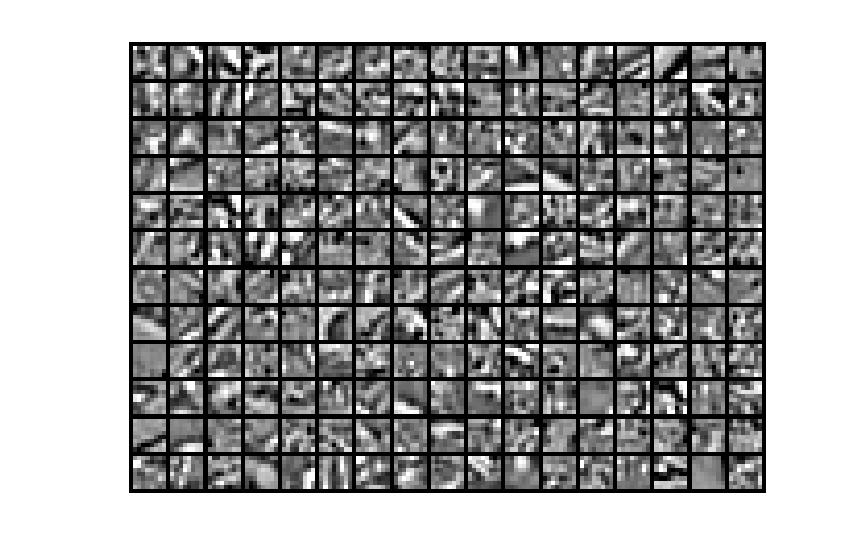
\includegraphics[scale = 0.5]{./imgs/SampleImage.jpg}
\noindent
Then we use file {\color{blue}\emph{\texttt{initializeParameters.m}}} to initialize parameters. As the number of input is just the same as the number of output, we only need two parameters to call this function.
We put \emph{hiddenSize = 25} and \emph{visibleSize = 64}, get the initialized parameters $\theta$ with shape $<3289\times1>$(64*25+64+25*62+25, each bias associates a neuron, input layer has bias and output layer has bias).\\
If you are already familiar with CNN and BP, then you know that our core function or our algorithm soul is to achieve cost function and compute its gradient. Dont't worry, you are unnecessarily afraid for it. In my point of view, it is much more easier than CNN's backpropagation, but still has some impressived equations we need to understand.
\begin{itemize}
\item {\color{blue}\emph{\texttt{spareAutoencoderCost.m}}}\\

\begin{table}[ht]
\caption{The variable space}
\centering
\begin{tabular}{c c|c c }
\hline
\rowcolor{blue!30} Variable Name & Value & variable Name & Value \\
\hline  
$theta$ & <3289*1> &$visibleSize$ & 64 \\ 
$hiddenSize$ & $25$ & $lambda$ & 1.0000e-04 \\ 
$sparsityParam$ & 0.0100 & beta & 3 \\
$data$ & <64*10000> & $W1$ & $<25\times64>$\\
$W2$ & $<64\times25>$ & $b1$ & $<25\times1>$\\
$b2$ & $<64\times1>$ & & \\
\hline 
\end{tabular}
\end{table}
\newpage
We use sigmoid function for activation function, and matrices $W^{(1)}\in\mathfrak{R}^{s_1\times s_2}$, $W^{(2)}\in\mathfrak{R}^{s_2\times s_3}$, vectors $b^{(1)}\in\mathfrak{R}^{s_2}$, $b^{(2)}\in\mathfrak{R}^{s_3}$. The objective $J_{sparse}(W,b)$ contains 3 terms, corresponding to squared error term, the weight decay term, and the sparsity penalty.\\
We write $\bm{a}_j^{(2)}\bm{(x)}$ to denote the activation of this hidden unit(unit $j$ in layer 2) when the network is given a specific input $\bm{x}$. Then the average activation of hidden unit $j$ (averaged over the training set) given as follow:
$$\hat{\rho}_j = \frac{1}{m}\sum_{i=1}^{m}\big[\bm{a}_j^{(x)}(\bm{x}^{(i)})\big]$$
If we use KL divergence(KL-divergence is a standard function for measuring how different two different distributions are.) and sum up all $\hat{\rho}_j$ in hidden layer, (in codes, \emph{mean\_act1} is $\hat{\rho_j}$ for all $j$, $\rho$ is \emph{sparsityParam}=0.0100), then
$$\sum_{j=1}^{s_2}\rho log\frac{\rho}{\hat{\rho}_j} + (1-\rho)log\frac{1-\rho}{1-\hat{\rho}_j}$$
and also can be written as
$$\sum_{j=1}^{s_2}\bm{KL}(\rho||\hat{\rho}_j)$$
For $W2grad$
$$\nabla_{\bm{W}^{(l)}}\bm{J(W,b;x,y)} = \delta^{(l+1)}(\bm{a}^{(l)})^T$$
$$\bm{W}^{(l)} = \bm{W}^{(l)} - \alpha\bigg[\bigg(\frac{1}{m}\Delta\bm{W}^{(l)} \bigg) + \lambda\bm{W}^{(l)}\bigg]$$
normally, we have 
$$\bm{\delta}^{(l)} = \Big((\bm{W}^{(l)})^T\bm{\delta}^{(l+1)}\Big)\bullet\bm{f'}(\bm{z}^{(l)})$$
now instead compute
$$\bm{\delta}_i^{(2)} = \Bigg( \bigg(\sum_{j=1}^{s_3}\bm{W}_{ji}^{(2)}\bm{\delta_j^{(3)}}\bigg)+ \beta\bigg(\frac{\rho}{\hat{\rho}_i} + \frac{1-\rho}{1-\hat{\rho}_i}\bigg)\Bigg)\bm{f'}(\bm{z}_i^{(2)})$$
In implementation, we will transmit \emph{delta1} to \emph{delta2}. Here \emph{delta1} is contacted layer 2, these codes may not will be denoted. Because for $\delta^{(l)}$ should from $n_l$(contacted layer $n_l$) to 2(contacted layer 2). After all, we just know, we use the privious $\delta$(suppose coming from layer $l$) and multiply the weigh $\bm{W}$ between layer $l$ and $l-1$.
\newpage
\begin{lstlisting}[caption = {backbone of spareAutoencoderCost.m}]
% numImages=10000
numImages = size(data,2);
numImages_inv = 1./numImages;
% for each image, we bind it a vector of bias vector b.
% note: we use all samples to compute, not a batch
% activations1 <25*10000> mean_act1 <25*1>
activations1 = sigmoid(W1*data+repmat(b1,[1,numImages]));
output = sigmoid(W2*activations1+repmat(b2,[1,numImages]));
mean_act1 = mean(activations1,2);
% squared_error <64*10000>
squared_error = 0.5.*(output - data).^2;
% squared error term, cost is a variable
cost = numImages_inv .* sum(squared_error(:));
% the weight decay term, cost is a variable
cost = cost + 0.5 .* lambda .* (sum(W1(:).^2) + sum(W2(:).^2));
% the sparsity penalty term, cost is a variable, after kl_div,
% will return <25*1>, and we just need to sum it up 
cost = cost + beta .* sum(kl_div(sparsityParam, mean_act1));
% delta2 <64*10000>
delta2 = -(data-output) .* output .* (1-output);
% gradient of bias in layer 2 connected layer 3: b2grad <64*1>
b2grad = mean(delta2,2);
W2grad = numImages_inv .* delta2 * activations1' + lambda .* W2;
% delta_sparsity <25*10000>, we use repmat to generate 10000 samples delta sparsity, 
% saying that for each sample, we really hope it has such a sparsity.
delta_sparsity = repmat(beta.*(-sparsityParam./mean_act1+(1-sparsityParam)./(1-mean_act1)), ...
[1,numImages]);
% delta2 <64*10000>, W2 <64*25>, delta1 <25*10000>
% delta1 has 25 rows, in hidden layer
delta1 = (W2' * delta2 + delta_sparsity) .* activations1 .* (1-activations1);
b1grad = mean(delta1,2);
% data in layer 1, is activation
W1grad = numImages_inv .* delta1 * data' + lambda .* W1;
grad = [W1grad(:) ; W2grad(:) ; b1grad(:) ; b2grad(:)];
\end{lstlisting}
At last, we use {\color{blue}\emph{\texttt{computeNumericalGradient.m}}} to check our cost function whether its computing process is correct or not. Then we use {\color{blue}\emph{\texttt{minFunc.m}}} to opitimize our cost function to get the \emph{opttheta} variable. Finally, we need to visualize $W1$. Because $\theta$ is consist of 4 parameters, $W1$, $W2$, $b1$, $b2$ successively.  
\begin{lstlisting}[caption = {Visualization}]
% W1 <25*64>
W1 = reshape(opttheta(1:hiddenSize*visibleSize), hiddenSize, visibleSize);
display_network(W1', 12); 
print -djpeg weights.jpg   % save the visualization to a file 
\end{lstlisting}
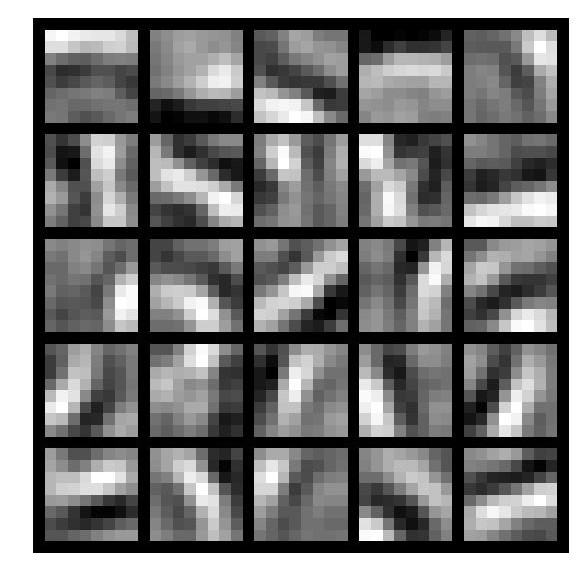
\includegraphics[scale = 0.8]{./imgs/weights.jpg}
\end{itemize}
\section{PCA, PCA Whitening and ZCA Whitening on Images}
For images, the input will be somewhat redundant, because the values of adjacent pixels in an image are highly correlated. We need a way to do dimensionality reduction and make features uncorrelated. The goal of whitening is to make the input less redundant; more formally, our desiderata are that our learning algorithms sees a training input where (i) the features are less correlated with each other, and (ii) the features all have the same variance. In detail, in order for PCA to work well, informally we require that (i) The features have approximately zero mean, and (ii) The different features have similar variances to each other. With natural images, (ii) is already satisfied even without variance normalization, and so we won’t perform any variance normalization. In this section, we only need a file {\color{blue}\emph{\texttt{pca\textunderscore gen.m}}}
\begin{itemize}
\item[1. ] For each image $\bm{x}^{(i)}$, we might normalize its the intensity as follows:
$$\mu^{(i)} := \frac{1}{n}\sum_{j=1}^{n}\bm{x}_j^{(i)}$$
$$\bm{x}_j^{(i)} := \bm{x}_j^{(i)} - \mu^{(i)} $$
for all $j$. \\
Here $i$ is to denoted images index, and $j$ is to denoted the $i$-th image $j$-th pixel intensity. 
\begin{lstlisting}[caption = {Zero-mean the data}]
% x is out input images set,<784*60000>, avg <1*60000>, a random 
% selection of 200 samples for visualization as follows
avg = mean(x,1);
x = x - repmat(avg,size(x,1),1);
\end{lstlisting}

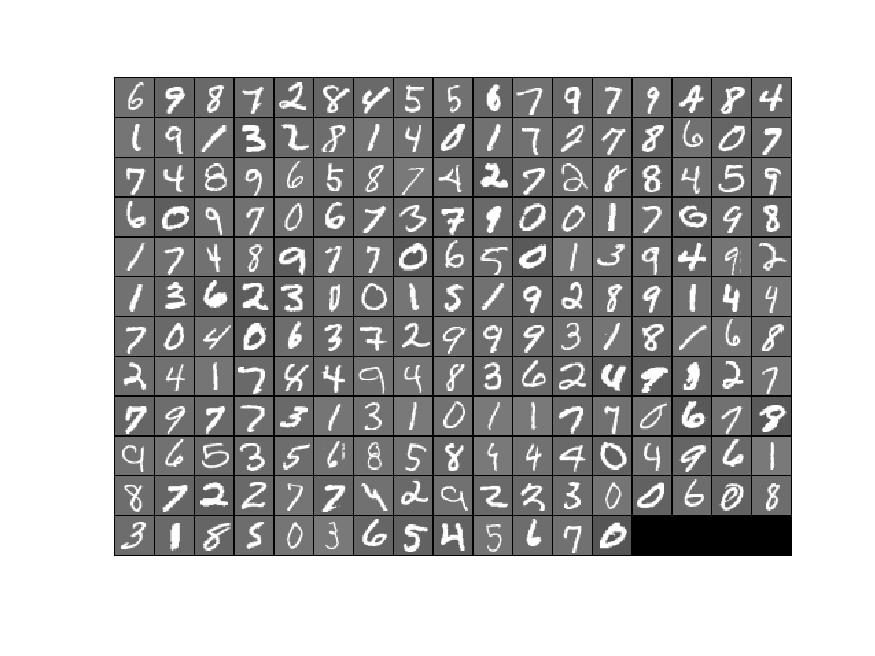
\includegraphics[scale = 0.5]{./imgs/displayimages.jpg}
\item[2. ] Next we need to compute the matrix $\Sigma$ defined as follows:
$$\Sigma = \frac{1}{m}\sum_{i=1}^{m}(\bm{x}^{(i)})(\bm{x}^{(i)})^T$$
If $\bm{x}$ has zero mean, then $\Sigma$ is exactly the covariance matrix of $\bm{x}$. In matlab, we can use  \emph{sigma = x * x' / size(x,2)}, which $x$ have m samples with shape $<n*m>$. (what is the relationship between the equation and matlab code? I am confused about it.) When we use Matlab \emph{svd} function, then the matrix U will contain the eigenvectors of Sigma (one eigenvector per column, sorted in order from top to bottom eigenvector), and the diagonal entries of the matrix S will contain the corresponding eigenvalues (also sorted in decreasing order). The matrix V will be equal to transpose of U, and can be safely ignored. The svd function actually computes the singular vectors and singular values of a matrix, which for the special case of a symmetric positive semi-definite matrix---which is all that we're concerned with here---is equal to its eigenvectors and eigenvalues. $\bm{x}_{rot}$(The subscript "rot" comes from the observation that this corresponds to a rotation (and possibly reflection) of the original data.) is another version of original data $\bm{x}$. If we get $\bm{x}_{rot}$, then we can go from the rotated vectors $\bm{x}_{rot}$ back to the original data $\bm{x}$ as follows:
$\bm{x} = \bm{U}\bm{x}_{rot}$

\begin{lstlisting}[caption = {Zero-mean the data}]
xRot = zeros(size(x)); % We need to compute this
% sigma <784*784>
sigma = x * x' / size(x,2); 
% u<784*784>, s<784*784>,v<784*784>
[u,s,v] = svd(sigma);
% xRot <784*10000>
xRot = u' * x; % rotated version of the data x
% If we want to a dimensioned version of original data, saying we 
% want to keep only k dimensions, use the follows statement, 
% where k is the number of eigenvectors to keep
% xTilde = U(:,1:k)' * x; 
\end{lstlisting}

\item[3. ] How can we insure that our xRot variable is right? Well, covariance matrix for the xRot should be a diagonal matrix with non-zero entries only along the main diagonal. So, we need to compute the covariance matrix of xRot and visualize it.
\begin{lstlisting}[caption = {Check your implementation of PCA}]
covar = zeros(size(x, 1)); % You need to compute this
covar = xRot * xRot' / size(xRot,2);
% Visualise the covariance matrix. You should see a line across the
% diagonal against a blue background.
figure('name','Visualisation of covariance matrix');
% you will see a coloured diagonal line against a blue background, 
% however, with so many samples, the diagonal line may not be apparent.
% you can check and see the concrete covar matrix in Matlab variables space
imagesc(covar);
\end{lstlisting}

\item[4. ] Now we need to decide how many dimensions should be retain. We will pick $k$ to be as small as possible, but so that at least 99\% of the variance is retained.
\begin{lstlisting}[caption = {Find k, the number of components to retain}]
k = 0; % Set k accordingly
% s contains our all eigenvalues
total = sum(s(:));
% mat <784*784>
mat = zeros(size(s,1));
% size(s,1) = 784
for i=1:size(s,1)
    mat(i,i) = 1;
    % s is a diagonal matrix, only diagonal has data.
    % In face, we just sum k elements in s in turn by diagonal and
    % compare the result to total sum to see the percentage
    res = mat * s;
    if (sum(res(:)) / total) >= 0.99
        break;
    end
end
k = i;
\end{lstlisting}

\item[5. ] We will recover our data with $k$ dimensions as follows:
\begin{lstlisting}[caption = {Implement PCA with dimension reduction}]
xHat = zeros(size(x));  % You need to compute this
u_k = u(:,1:k); % <784*300>
xHat = u_k * u_k' * x; % x <784*60000>
figure('name',['PCA processed images',sprintf('(%d / %d dimensions)', k, size(x, 1)),'']);
display_network(xHat(:,randsel));
figure('name','Raw images');
display_network(x(:,randsel))
\end{lstlisting}
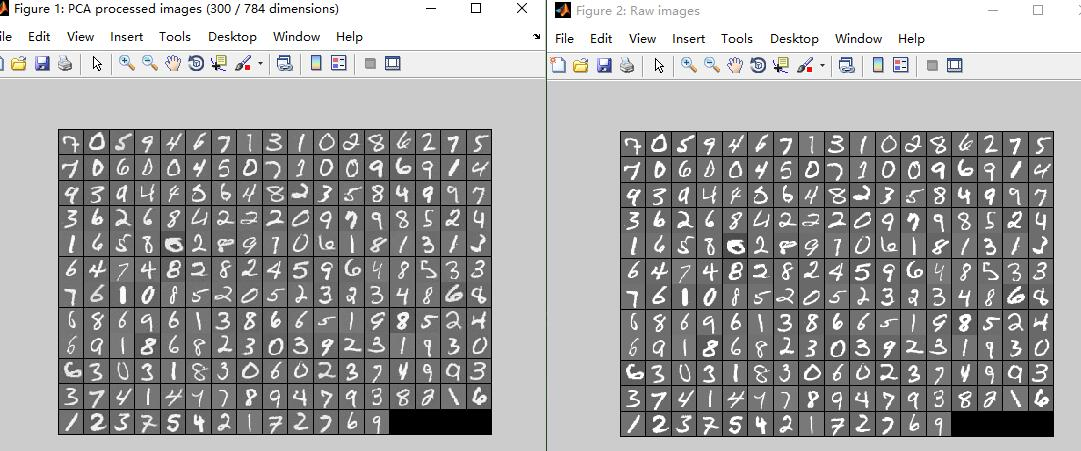
\includegraphics[scale = 0.6]{./imgs/pca2.jpg}


\item[6. ] PCA whitening and regularisation.
\begin{lstlisting}[caption = {Implement PCA with whitening and regularisation}]
% Without regularisation (set epsilon to 0 or close to 0), 
epsilon = 0.1;
xPCAWhite = zeros(size(x));
% As we have compute, xRot = u' * x; xPCAWhite <784*60000>
xPCAWhite = diag(1./sqrt(diag(s)+epsilon)) * xRot;

% use the dimensioned x to do pca whitening
% xPCAWhite_rd = diag(1./sqrt(diag(s)+epsilon)) * u' * xHat;

%  Check our implementation of PCA whitening with and without regularisation. 
%  PCA whitening without regularisation results a covariance matrix 
%  that is equal to the identity matrix. PCA whitening with regularisation
%  results in a covariance matrix with diagonal entries starting close to 
%  1 and gradually becoming smaller
covar = xPCAWhite * xPCAWhite' / size(xPCAWhite,2);
figure('name','Visualisation of covariance matrix');
imagesc(covar);
\end{lstlisting}
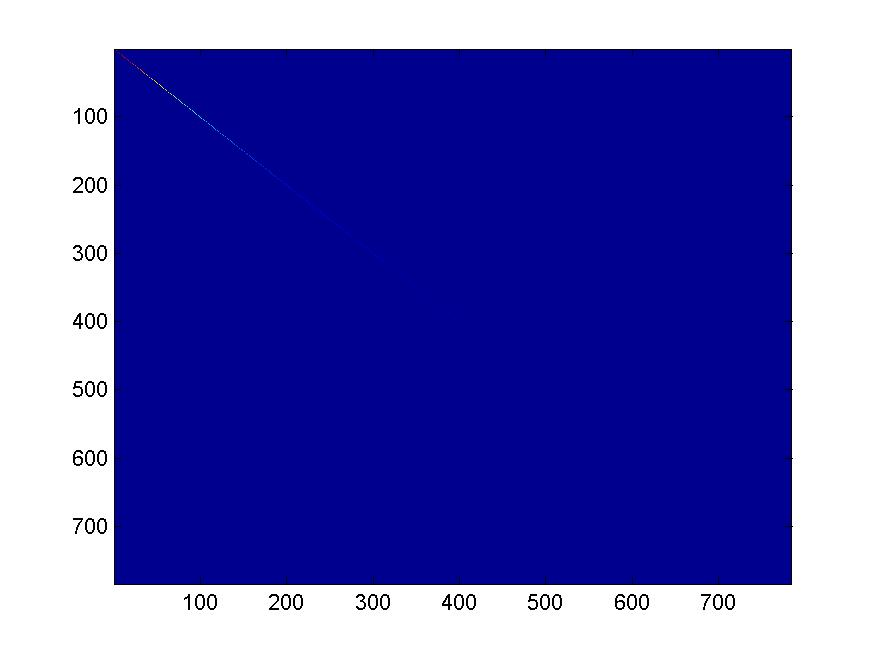
\includegraphics[scale = 0.4]{./imgs/pcaWhitening.jpg}
\item[7. ] 
\begin{lstlisting}[caption = {Implement ZCA whitening}]
xZCAWhite = zeros(size(x));
% xZCAWhite <784*60000>
xZCAWhite = u * xPCAWhite;
% Visualise the data, and compare it to the raw data.
% You should observe that the whitened images have enhanced edges.
figure('name','ZCA whitened images');
display_network(xZCAWhite(:,randsel));
figure('name','Raw images');
display_network(x(:,randsel));
\end{lstlisting}
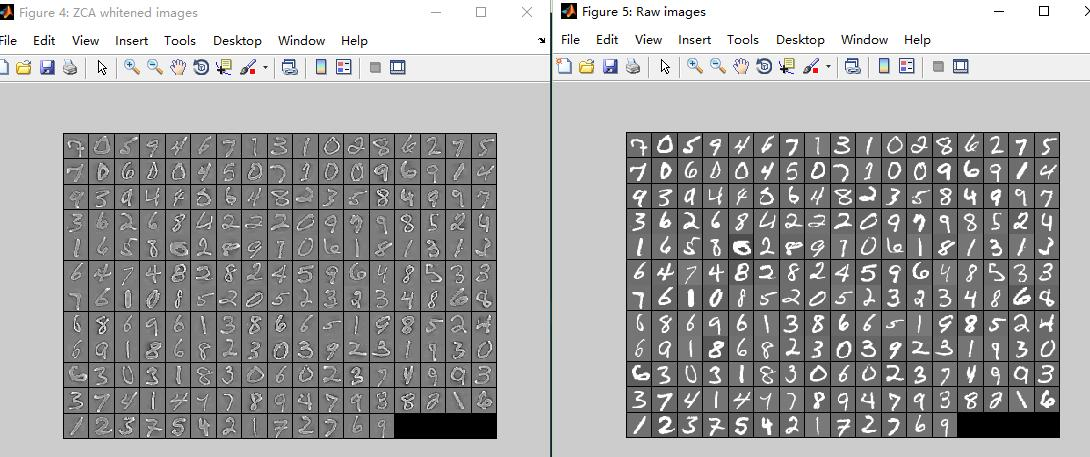
\includegraphics[scale = 0.5]{./imgs/ZCA.jpg}
\end{itemize}
\newpage

\section{Reconstruction ICA}
Independent Component Analysis (ICA) allows us to generate sparse representations of whitened data. But ICA, has difficulties arise when the number of features (rows of $\bm{W}$ matrix), exceed the dimensionality of input, $\bm{x}$.
\section{Self-raught Learning}
I have not completed it, but I know its principles.


\end{document}
